\documentclass[reprint,prb,superscriptaddress]{revtex4-2}
\usepackage{braket,amsmath,graphicx,float,color,ulem,soul,lipsum}
\usepackage[hidelinks]{hyperref}
\bibliographystyle{apsrev4-1}
\begin{document}

\title{Local metal-insulator transition in a generalised impurity Anderson model}
\author{Abhirup Mukherjee}
\email{am18ip014@iiserkol.ac.in }
\affiliation{Department of Physical Sciences, Indian Institute of Science Education and Research-Kolkata, W.B. 741246, India}
\author{Siddhartha Lal}
\email{slal@iiserkol.ac.in}
\affiliation{Department of Physical Sciences, Indian Institute of Science Education and Research-Kolkata, W.B. 741246, India}

\date{\today}

\begin{abstract}

\end{abstract}

\maketitle

%\tableofcontents

\section{Introduction}

The Hubbard model is one of the fundamental models for strong electronic correlation; in its simplest form, it features a single band of conduction electrons hopping on a lattice and interacting via local correlations that provide a cost \(U\) if any site is doubly occupied:
\[H_\text{hubb} = -t\sum_{\left<i,j \right>,\sigma}\left(c^\dagger_{i\sigma}c_{j\sigma}+\text{h.c.}\right) + U\sum_i \hat n_{i \uparrow} \hat n_{i \downarrow} - \mu \sum_{i,\sigma}\hat n_{i\sigma}\]
The model can be made particle-hole symmetric by choosing \(\mu = U/2\):
\[H_\text{hubb} = -t\sum_{\left<i,j \right>,\sigma}\left(c^\dagger_{i\sigma}c_{j\sigma}+\text{h.c.}\right) - \frac{U}{2}\sum_i \left(\hat n_{i \uparrow} - \hat n_{i \downarrow}\right)^2\]
There are two trivial limits of the model. At \(U=0\), the bath consists of just a kinetic energy part, and the ground state is just a filled Fermi sea. At \(t=0\), each lattice site decouples from the rest and becomes a local moment, which under symmetry-breaking becomes a Neel antiferromagnet. This suggests that on increasing \(U/t\) beyond some critical value, the system might undergo a phase transition from a metallic state to an insulating state~\cite{Mott_1949}. This transition is reflected in the local spectral function - while it has a well-defined zero energy peak in the metallic phase, it is gapped in the insulating phase.

One method of studying Hubbard models is through auxiliary models, described in the next section. Auxiliary models are simpler versions of the full Hamiltonian that are able to capture the essential physics. For eg, a correlated impurity interacting with a conduction bath is a potential auxiliary model for the Hubbard Hamiltonian:
The impurity has onsite energy \(\epsilon_d\) and an onsite correlation \(U\). It hybridises into the bath through \(V\).

If the impurity site hybridises with a {\it non-interacting} bath defined by a uniform density of states, the impurity spectral function is found to have a well-defined Kondo resonance at low temperatures. Increasing the impurity correlation \(U\) only serves to reduce the width of the central peak at the cost of the appearance of side bands at energy scales of the order of \(U\), but the resonance never dies. The situation is however different if the impurity is embedded in a correlated conduction bath with a non-trivial density of states. For the case of a conduction band with the DOS shown in the right of the figure below, the impurity hybridises into a reduced bandwidth because of the correlation on the lattice~\cite{held_2013}.

This difference in the type of conduction baths is utilized in dynamical mean-field theory to describe various phases of the bulk system.
This is done through the DMFT algorithm: one starts with a non-interacting bath, but depending on the value of \(U\), the conduction bath then gets modified and we ultimately end up with something that is different from what we started with.
For small \(U\), the bath does not change much and we retain the central resonance of the impurity spectral function.
This then describes a metal in the bulk.
For larger values of \(U\), however, the bath changes significantly such that its density of states becomes non-constant.
Above a critical \(U_c\), the impurity spectral function gets gapped out, and that then describes the insulating phase in the bulk.
\textit{This leaves open the following question}: What is the minimal correlation one can insert into the non-interacting bath (of a single-impurity Anderson model) that can capture both the metallic and insulating phases of the bulk model?

\begin{figure}[!htb]
\centering
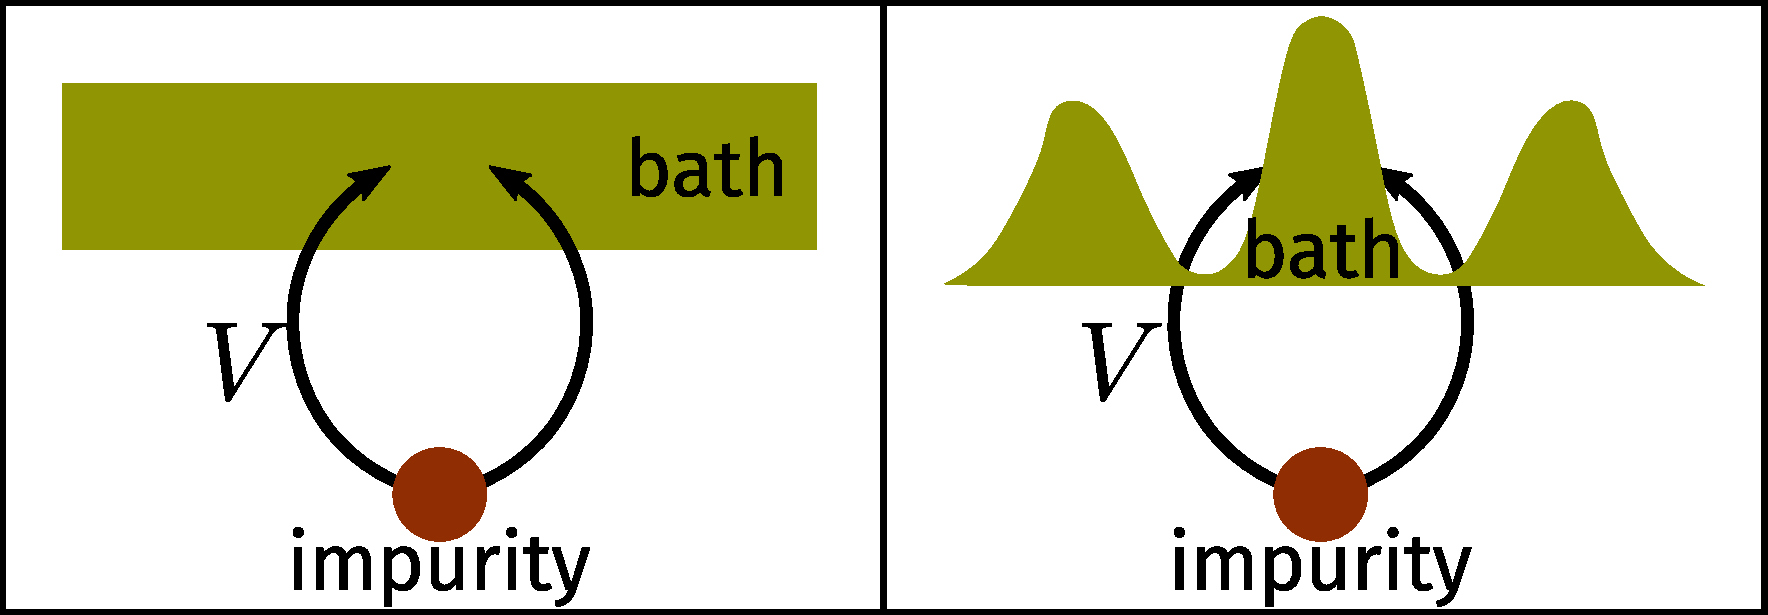
\includegraphics[width=0.5\textwidth]{../figures/dos_diff.pdf}
\caption{Two kinds of bath that an impurity can hybridise into. The left panel shows a non-interacting conduction band with a flat density of states. The right panel shows an interacting bath with an energy-dependent density of states. In the latter case, the impurity "feels" a reduced effective bandwidth defined by the width of the central peak.}
\end{figure}

\section{The generalised Anderson impurity model}

The impurity models we will work with couple the impurity to a single site in the lattice. We will refer to that specific site as the zeroth site throughout. We recall the Hamiltonian of the Anderson impurity model with a half-filled impurity site:
\begin{equation} 
	\mathcal{H} = \frac{- U}{2} \left(\hat n_{d \uparrow} - \hat n_{d \downarrow}\right)^2 + \sum_{\vec k,\sigma} \epsilon_{\vec k} \tau_{\vec k,\sigma} + V\sum_\sigma \left( c^\dagger_{d\sigma}c_{0\sigma} + \text{h.c.}\right)~,
 \end{equation}
where \(\tau_{\vec k,\sigma} \equiv \hat n_{\vec k,\sigma} - 1/2\). Also, \(c_{d\sigma}\) and \(c_{0\sigma}\) are the fermionic annihilation operators of spin \(\sigma\) for the impurity and zeroth sites respectively. \(U\) is the repulsive correlation on the impurity site, and the impurity is at particle-hole symmetry. \(V\) is the momentum-independent hybridisation parameter that couples the impurity with the lattice. We will work with a constant density of states in the bath. 


In order to enhance the Anderson impurity model, we introduce two extra two-particle interaction terms into the Hamiltonian:
\begin{itemize}
	\item a spin-exchange term \(J \vec{S}_d\cdot\vec{s}_0\) between the impurity spin \(\vec S_d\) and the spin \(\vec s_0\) of the zeroth site 
	\item a local correlation term \(U_b \hat n_{0 \uparrow} \hat n_{0 \downarrow}\) on the zeroth site
\end{itemize}

With these additional terms, the generalised Anderson impurity model, at particle-hole symmetry, is
\begin{equation}\begin{aligned}
	\mathcal{H} = \frac{- U}{2} \left(\hat n_{d \uparrow} - \hat n_{d \downarrow}\right)^2 + \sum_{\vec k,\sigma} \epsilon_{\vec k} \tau_{\vec k,\sigma} + V\sum_\sigma \left( c^\dagger_{d\sigma}c_{0\sigma} + \text{h.c.}\right)\\
	+ J \vec{S}_d\cdot\vec{s}_0 + U_b \hat n_{0 \uparrow} \hat n_{0 \downarrow}
\end{aligned}\end{equation}
All the terms in the Hamiltonian have been depicted schematically in fig.~\ref{zeromode-bare}.

\begin{figure}[!htb]
	\centering
	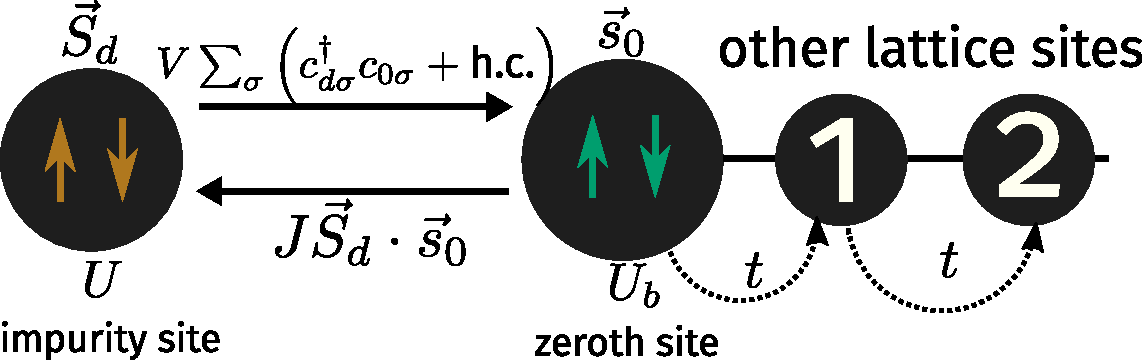
\includegraphics[width=0.45\textwidth]{../figures/zeromode_bare.pdf}
	\caption{While we have studied the full model under renormalisation group, often we will turn to a simplified zero-bandwidth version of the model that is obtained by ignoring the kinetic energy part of the Hamiltonian. This zero-bandwidth model is effectively a two site model.}
	\label{zeromode-bare}
\end{figure}

\section{RG Equations for the model}
We now perform a renormalisation group analysis of the MCK Hamiltonian using the recently developed URG method \cite{anirbanmott1,anirbanmott2,anirbanurg1,anirbanurg2,siddharthacpi,santanukagome,1dhubjhep}.
The RG proceeds {by applying unitary transformations in order to block-diagonalize the Hamiltonian by removing number fluctuations of the high energy degrees of freedom}.
Given the most energetic electronic state at the \(j^\text{th}\) RG step is \(\ket{j}\) and defined by the energy \(D_{(j)}\), the Hamiltonian will in general not conserve the number of particles in this state: \(\left[H_{(j)}, \hat n_{j}\right] \neq 0\).
The unitary transformation \(U_{(j)}\) will remove this number fluctuation at the next RG step~\cite{anirbanurg1,anirbanurg2}:
\begin{equation}\begin{aligned}
	H_{(j-1)} = U_{(j)} H_{(j)} U^\dagger_{(j)}~, ~\left[H_{(j-1)}, \hat n_{j}\right] =0~.
\end{aligned}\end{equation}
The unitary transformations are given in terms of a fermionic generator \(\eta_{(j)}\)~\cite{anirbanurg1,anirbanurg2}:
\begin{equation}\begin{aligned}
	U_{(j)} = \frac{1}{\sqrt 2}\left(1 + \eta_{(j)} - \eta_{(j)}^\dagger\right)~,~ \quad\left\{ \eta_{(j)},\eta_{(j)}^\dagger \right\}_\pm = 1~,
\end{aligned}\end{equation}
where \(\left\{A,B\right\}_\pm = AB \pm BA\). The generator itself is given by the expression~\cite{anirbanurg1,anirbanurg2}
\begin{equation}\begin{aligned}
	\eta^\dagger_{(j)} = \frac{1}{\hat \omega_{(j)} - \text{Tr}\left(H_{(j)} \hat n_{j}\right) } c^\dagger_{j} \text{Tr}\left(H_{(j)}c_{j}\right)~.
\end{aligned}\end{equation}
The operator \(\hat \omega_{(j)}\) encodes the quantum fluctuation scales arising from the interplay of the kinetic energy terms and the interaction terms in the Hamiltonian:
\begin{equation}\begin{aligned}
	\hat \omega_{(j)} = H_{(j-1)} - H^i_{(j)}~.
\end{aligned}\end{equation}
\(H^i_{(j)}\) is that part of \(H_{(j)}\) that commutes with \(\hat n_j\) but does not commute with at least one \(\hat n_l\) for \(l < j\). The RG flow continues up to energy \(D^*\), where a fixed point is reached from the vanishing of the RG function. 

The derivation of the RG equations for the generalised Anderson impurity model Hamiltonian is shown in the appendix. We provide below the RG equations for a given quantum fluctuation scale \(\omega\):
\begin{gather}
	\Delta U_b = 0~,\\
	\Delta U = 4V^2 n_j\left(\frac{1}{d_1} - \frac{1}{d_0}\right) - n_j\frac{J^2}{d_2}~,\\
	\Delta V = -\frac{3n_j V}{8}\left[J\left(\frac{1}{d_2} + \frac{1}{d_1}\right) +  \frac{4U_b}{3}\sum_{i=1}^4 \frac{1}{d_i}\right]~,\\
	\Delta J = -\frac{n_j J\left(J + 4U_b\right)}{d_2}~.
\end{gather}
The denominators \(d_i\) used in these equations are given by
\begin{gather}
	d_0 = \omega - \frac{D}{2} + \frac{U_b}{2} - \frac{U}{2}~,\\
	d_1 = \omega - \frac{D}{2} + \frac{U_b}{2} + \frac{U}{2} + \frac{J}{4}~,\\
	d_2 = \omega - \frac{D}{2} + \frac{U_b}{2} + \frac{J}{4}~,\\
	d_3 = \omega - \frac{D}{2} + \frac{U_b}{2}~.
\end{gather}
The symbols used in the RG equations have the following meanings: \(\Delta U\) represents the renormalisation in the coupling \(U\) in going from the \(j^\text{th}\) Hamiltonian to the \(\left( j-1 \right) ^\text{th}\) Hamiltonian by decoupling the isoenergetic shell at energy \(D_{(j)}\). \(n_j\) is the number of electronic states on the shell \(D_{(j)}\).

We will discuss the consequences of these RG equations in the next sections, but we clarify here that the labels \(U_0,J_0,V_0\) that will occur in the axes of the plots or anywhere else represent the bare values of the couplings \(U,J\) and \(V\). We also point out here that throughout the upcoming results, the bare value of \(U_b\) is set to the negative of the bare value of \(U_0\): \(U_b = -U_0/10\). This means that whenever we vary \(U_0\) along the axis of a plot, we are simultaneous varying \(U_b\).	The reason for choosing the negative sign of \(U_b\) will be clarified in the next section.

\section{RG flows and phase diagram}

We start the discussion on the nature of the RG flows by pointing out the spin-exchange coupling \(J\) has a critical point \(\left( \Delta J = 0 \right) \) at \(U_b = -J/4\). Since \(J\) is positive, this means that we can capture both relevant and irrelevant RG flows of \(J\) by keeping \(U_b\) negative. \(U_b\) is found to be marginal under the RG transformation, and we set \(U_b\) to \(-U_0/10\) hereafter. We will work in the regime of quantum fluctuations where all the denominators are negative: \(d_i < 0 ~\forall~i\).

\subsection{RG flows for \(4U_b + J > 0\)}

\begin{figure}[htpb]
	\centering
	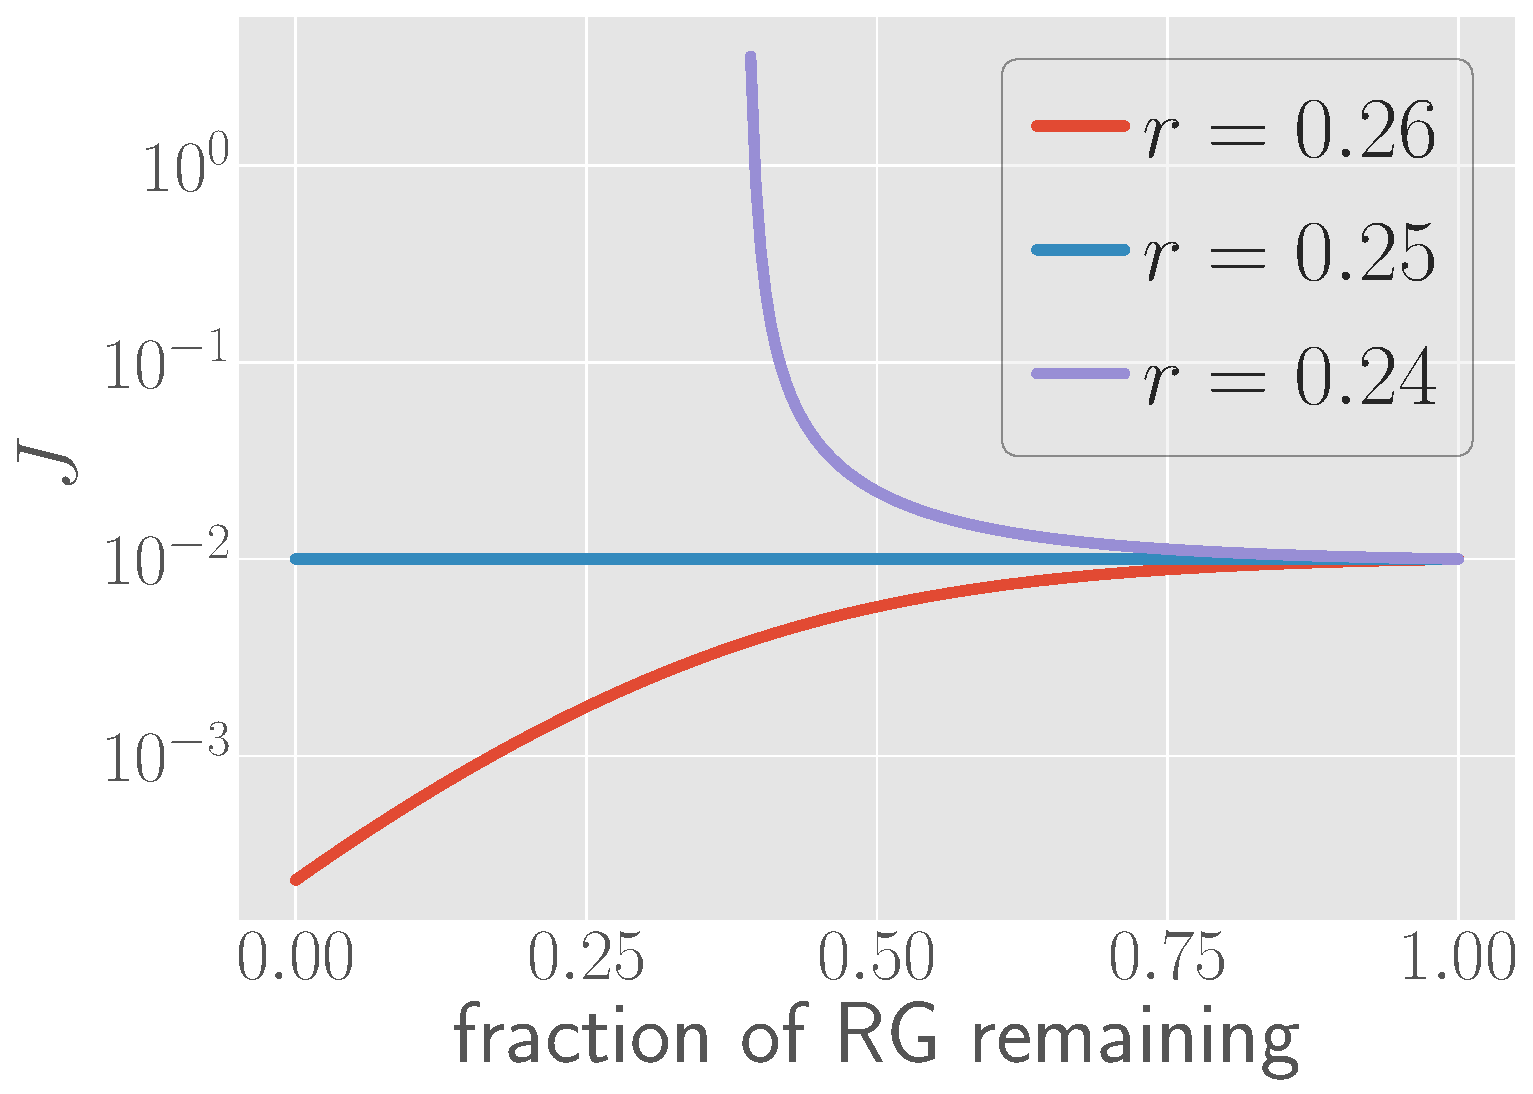
\includegraphics[width=0.45\textwidth]{../figures/J_Ub.pdf}
	\caption{JUb}
	\label{fig:-figures-J_Ub-pdf}
\end{figure}
\begin{figure}[htpb]
	\centering
	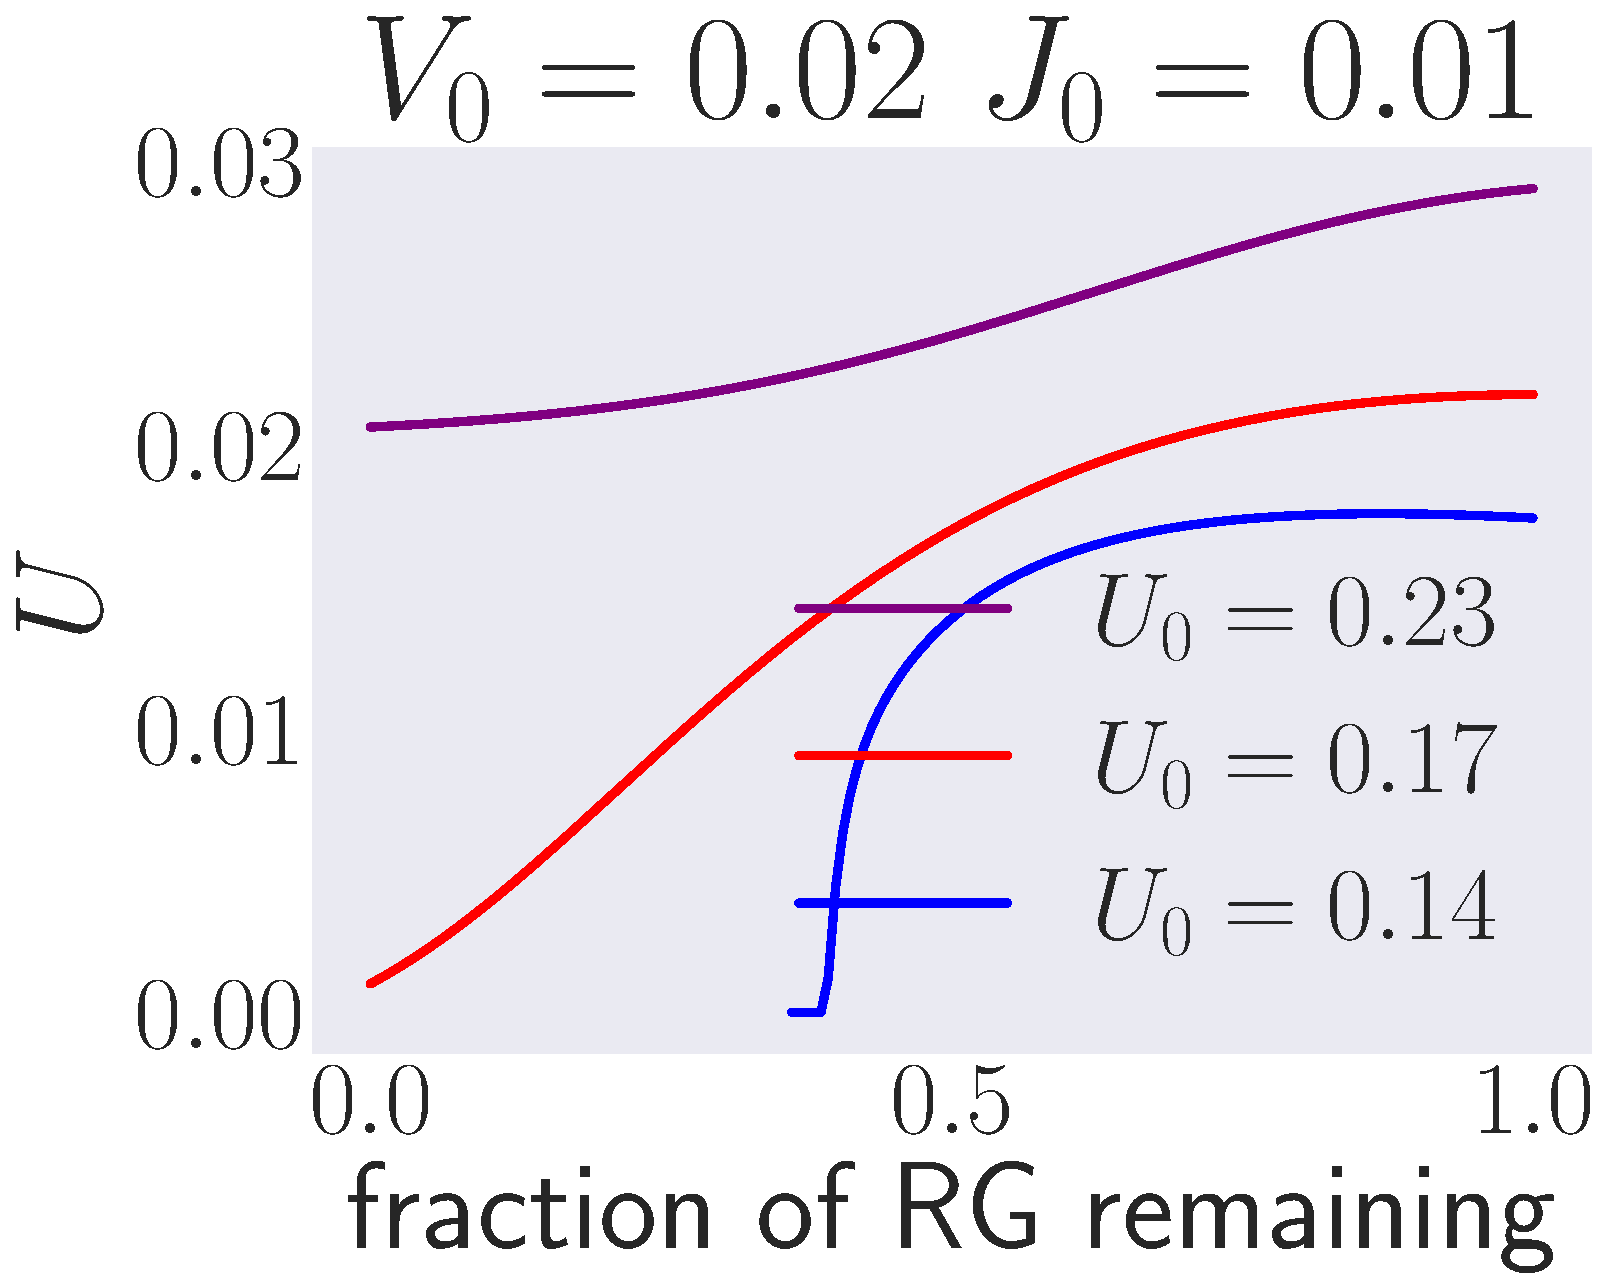
\includegraphics[width=0.45\textwidth]{../figures/U_Ub.pdf}
	\caption{JUb}
	\label{fig:-figures-J_Ub-pdf}
\end{figure}

\begin{widetext}

\begin{figure}[!htb]
	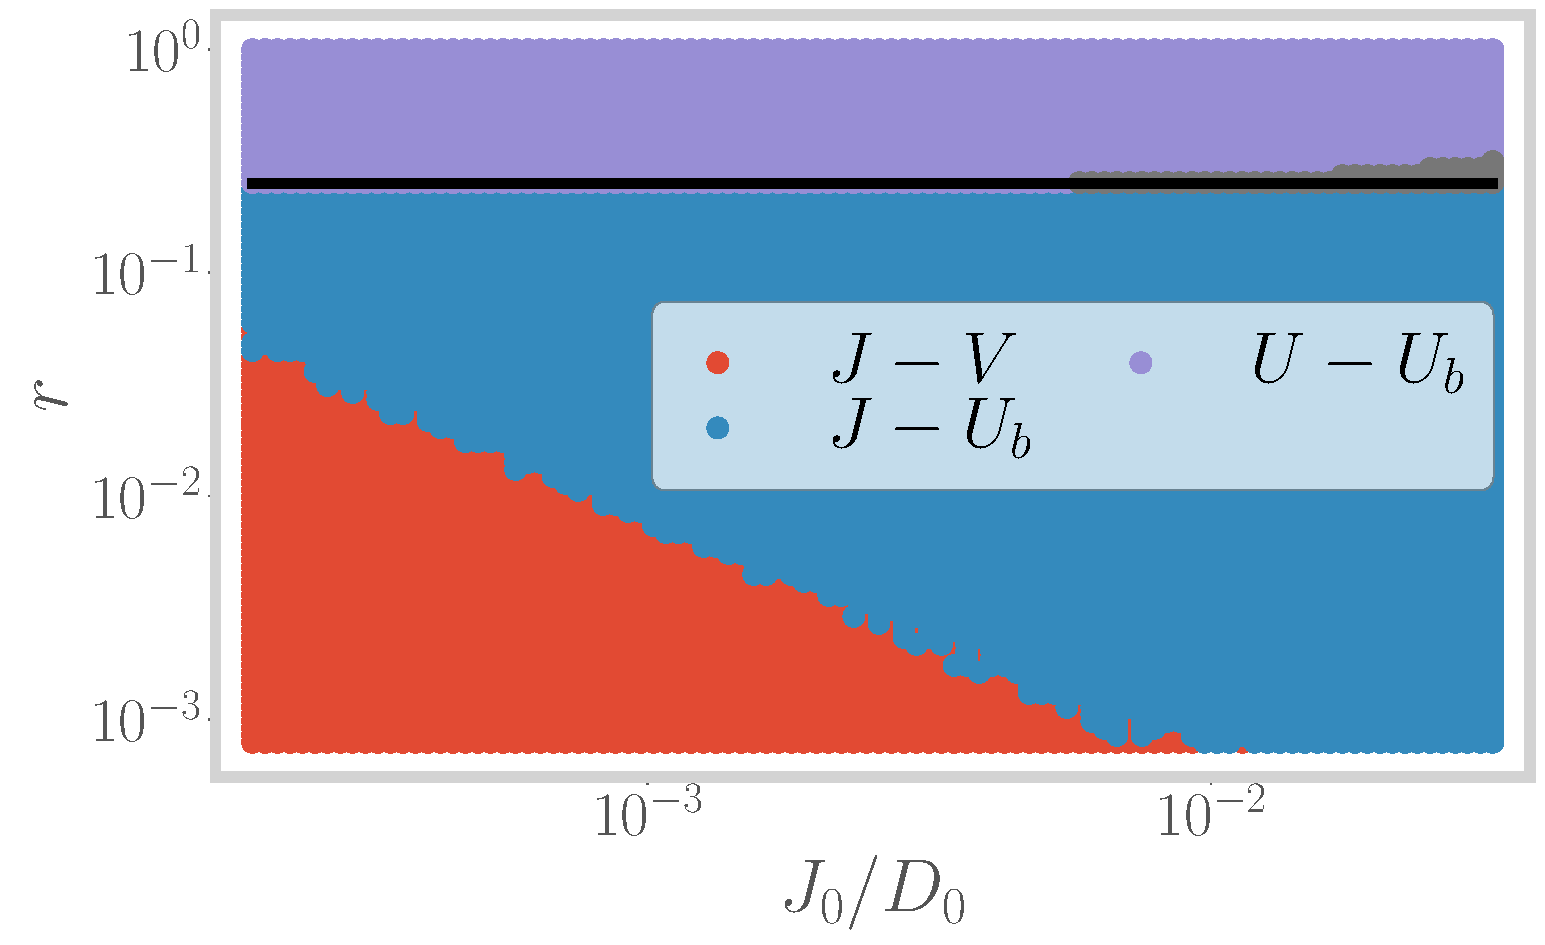
\includegraphics[width=0.7\textwidth]{../figures/phase-map-MIT.pdf}
\end{figure}

\end{widetext}
\begin{table}
\centering
\begin{tabular}{|c|c|c|c|c|}
\hline
phase & RG flow & fixed point & GS & 2-site GS \\ 
\hline
blue & \(\Delta U <0, \Delta J,\Delta V>0\) & \(U^* \ll V^* \ll J^*\) & SS & \(\ket{SS}=\ket{\uparrow,\downarrow} - \ket{\downarrow, \uparrow}\)  \\ 
green &  \(\Delta U < 0, \Delta J < 0,\Delta V>0\) & \(J^* < U^* \ll V^*\) & SS + CT-0 & \(c\ket{SS} + \sqrt{1-c^2}\ket{CT-0}\)  \\  
red &  \(\Delta U > 0, \Delta J,\Delta V<0\) & \(U^* \gg 1,  V^* = J^* = 0\) & decoupled LM & \(\left\{\ket{\uparrow}, \ket{\downarrow} \right\} \otimes \left\{\ket{0}, \ket{2}\right\} \) \\
gray &  \(\Delta U, \Delta J,\Delta V < 0\) & \(U^* = V^* = J^* = 0\) & lattice & \(\left\{\ket{\uparrow}, \ket{\downarrow}, \ket{0}, \ket{2} \right\} \otimes \left\{\ket{0}, \ket{2}\right\}\) \\
\hline
\end{tabular}
\end{table}

\section{Low-energy effective Hamiltonian and the ground state}

\subsection{Screened regime: \(-U_b/J < 1/4 \)}

The fixed point Hamiltonian can, in general, be written as
\begin{equation}\begin{aligned}
	\mathcal{H}^* = \sum_{\sigma, k}\epsilon_k \tau_{k\sigma} - \frac{U^*}{2}\left(\hat n_{d \uparrow} - \hat n_{d \downarrow}\right)^2  + \sum_{\sigma, k < \Lambda^*}\left( V^* c^\dagger_{k\sigma}c_{d\sigma} + \text{h.c.} \right) + J^* \vec{S_d}\cdot\vec{s}
\end{aligned}\end{equation}
The first term is the kinetic energy of all the electrons. The next two terms are the impurity-diagonal pieces, featuring the renormalised interaction \(U^*\). The next three terms are the residual interactions between the impurity and the metal, with the renormalised couplings \(V^*, J^*\) and \(K^*\). The summations in these terms extend from the fixed point momentum cutoff \(\Lambda^*\) to 0. This is the region of momentum space  which the URG was unable to decouple. The operators \(\vec s\) and \(\vec C\) represent the macroscopic magnetic and charge spins formed by the remaining electrons that are lying inside the window \(\left[ 0, \Lambda^* \right] \):
\begin{equation}\begin{aligned}
	\vec s = \sum_{kk^\prime<\Lambda^*\atop{\alpha\beta}} c^\dagger_{k\alpha}\vec \sigma_{\alpha\beta}c_{k^\prime\beta}
\end{aligned}\end{equation}
Our goal here is to write down the ground state wavefunction for this low-energy Hamiltonian.

To make progress, we will simplify the effective Hamiltonian by taking the zero bandwidth limit. This reduces it to a two-site problem. One site is of course the impurity site, and this site will be labeled as site 1. The other site will be formed by the center of mass degree of freedom of the conduction electrons, and will be labeled as site 2. The Hamiltonian for this two-site problem is
\begin{equation}\begin{aligned}
	\mathcal{H}_{IR} = - \frac{U^*}{2}\left(\hat n_{1 \uparrow} - \hat n_{1 \downarrow}\right)^2 + V^*\sum_{\sigma}\left(c^\dagger_{1\sigma}c_{2\sigma} + \text{h.c.} \right) + J^*\vec{S_1}\cdot\vec{S_2} + K^* \vec{C_1}\cdot\vec{C_2}
\end{aligned}\end{equation}


The subscripts on the operators designate the site on which they act; \(\hat n_1\) is the number operator for the first site.

We will adopt the following notation to represent the states in this Hilbert space. A general state will be represented in the Fock space basis as \(\ket{n_{1 \uparrow}n_{1 \downarrow}n_{2 \uparrow}n_{2 \downarrow}}\). For example,
\begin{equation}\begin{aligned}
	\ket{1101} = c^\dagger_{1 \uparrow}c^\dagger_{1 \downarrow}c^\dagger_{2 \downarrow}\ket{-}
\end{aligned}\end{equation}
\(\ket{-}\) is the vacuum state.

For \(U>0\), the ground state is given by
\begin{gather}
	\label{gstate}
	\ket{\Psi}_\text{1} = c_s \frac{1}{\sqrt 2}\left(\ket{\uparrow, \downarrow} - \ket{\downarrow, \uparrow}\right) + c_c \frac{1}{\sqrt 2}\left(\ket{\uparrow\downarrow, 0} + \ket{0, \uparrow\downarrow}\right), \quad E_1 =  -V^*\sqrt{\gamma^2 + 4} -\frac{1}{4}U^* - \frac{3}{8}{J^*}
\end{gather}
where $\gamma = \frac{1}{2{V^*}}\left[ \frac{1}{4}\left( 3J^* + K^* \right) + \frac{1}{2}U^* \right]$. The probabilities for the spin and charge sectors for the ground state are
\begin{equation}\begin{aligned}
	\label{coeff_def}
	\left(c_s\right)^2 = \frac{1}{2\sqrt{\gamma^2 + 4}}\left(\sqrt{\gamma^2 + 4} + \gamma\right),\\
	\left(c_c \right)^2 = \frac{1}{2\sqrt{\gamma^2 + 4}}\left(\sqrt{\gamma^2 + 4} - \gamma\right)~.
\end{aligned}\end{equation}
For (roughly) \(J_0 > V_0\), we get \(J^* \gg V^*\) and \(U^* \gg U_0\) so that \(\gamma \gg 1\). This gives \(\left( c_s \right) ^2 \sim 1\) and \(\left( c_c \right) ^2 \sim 0\). The entire contribution to the ground state then comes from the spin sectors of the two sites. This is calculated numerically in fig.~\ref{cs_cc}.
\begin{figure}[!htb]
	\centering
	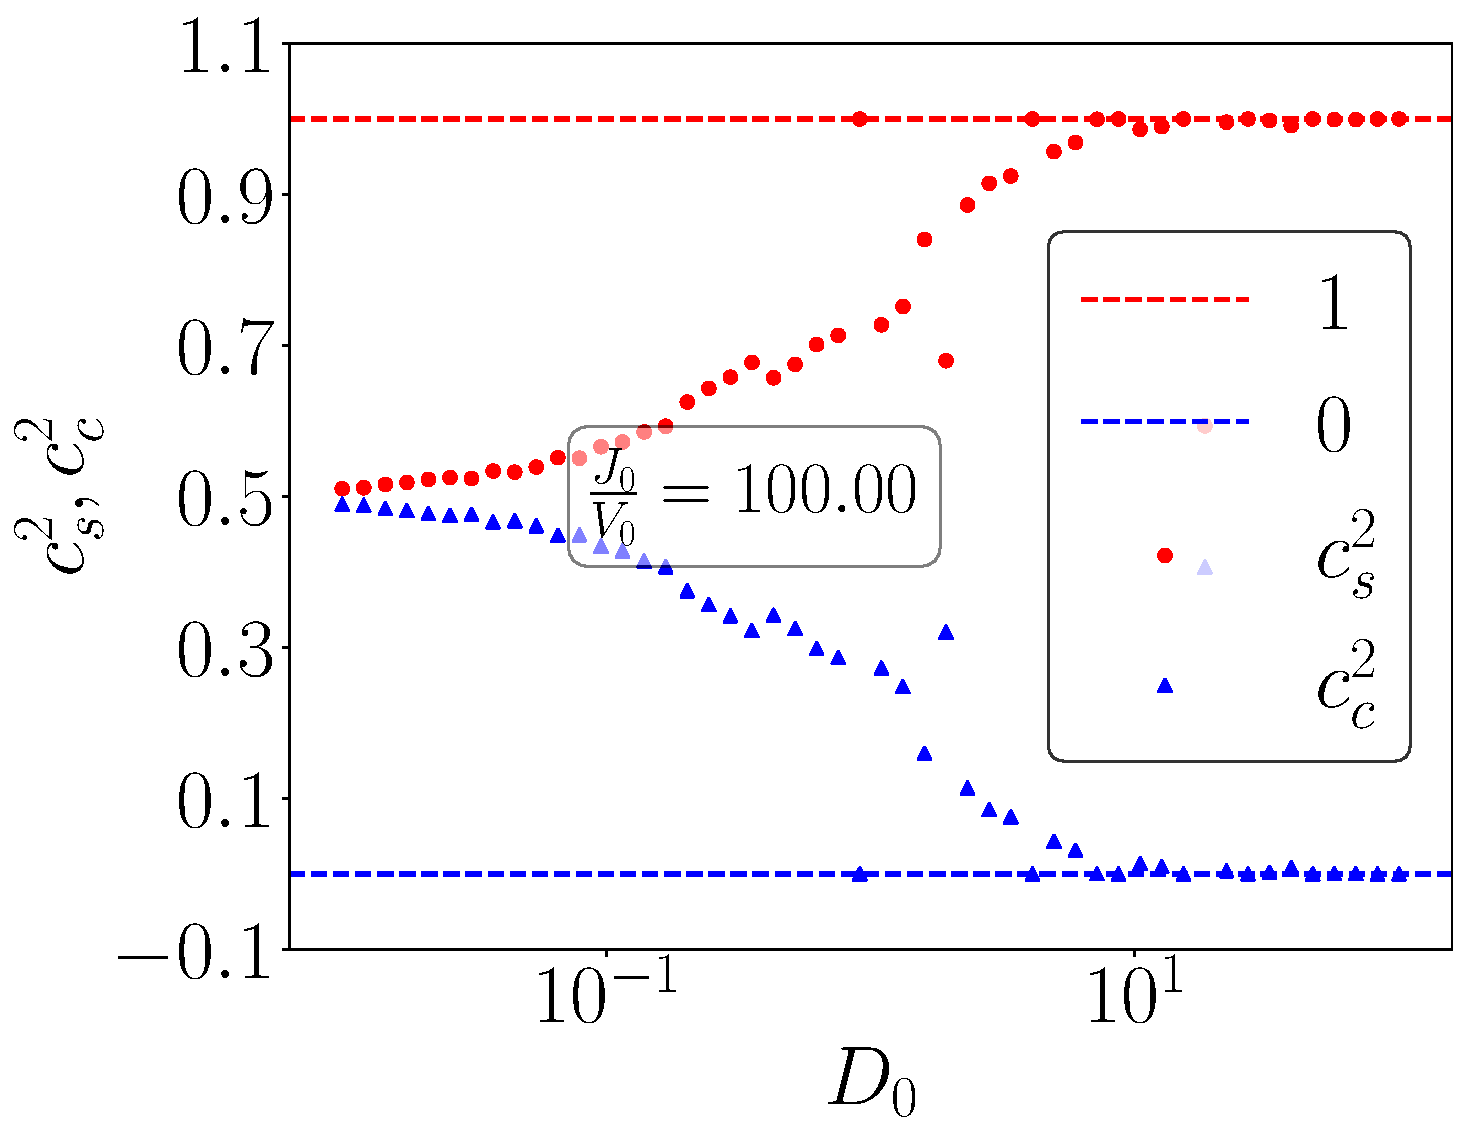
\includegraphics[width=0.5\textwidth]{../figures/coeffs_vs_J.pdf}
	\caption{Variation of relative weights \(c_s\) and \(c_c\) with \(J_0\)}
	\label{cs_cc}
\end{figure}

In the other regime of \(U<0\), the two competing states are \(\ket{\Psi}_1\) defined above (with energy \(E_1\)), and \(\ket{\Psi_2}\), the charge singlet: \(\ket{\Psi}_2 = \frac{1}{\sqrt 2}\left( \ket{2,0} - \ket{0,2} \right)\) having energy \(E_2\).
\begin{equation}\begin{aligned}
	E_2 = -\frac{3}{4}K^*, \quad E_1 - E_2 = -\frac{1}{4}\sqrt{\left( \frac{1}{2}K^* + U^* \right)^2 + (4V^*)^2} - \frac{1}{4}U^* + \frac{3}{4}K^*
\end{aligned}\end{equation}
For \(V_0 \gg K_0\), the largest energy scale will be \(V^*\), and we can then approximate this difference as
\begin{equation}\begin{aligned}
	E_1 - E_2 \simeq -V^* < 0
\end{aligned}\end{equation}
In such a case, \(\ket{\Psi}_1\) will therefore be the ground state. In the other regime \(V_0 \ll K_0\), the largest energy scale will be \(K^*\), and we can then write
\begin{equation}\begin{aligned}
	E_1 - E_2 \simeq - \frac{1}{8}K^* + \frac{3}{4}K^* > 0
\end{aligned}\end{equation}
In this case, the ground state will be \(\ket{\Psi}_2\). There exists, therefore, a phase transition at a critical plane \((U_c, K_c, V_c)\), where the ground state changes between the charge singlet \(\ket{\Psi}_2\) and the spin singlet + charge triplet \(\ket{\Psi}_1\).
\begin{figure}[!htb]
	\centering
	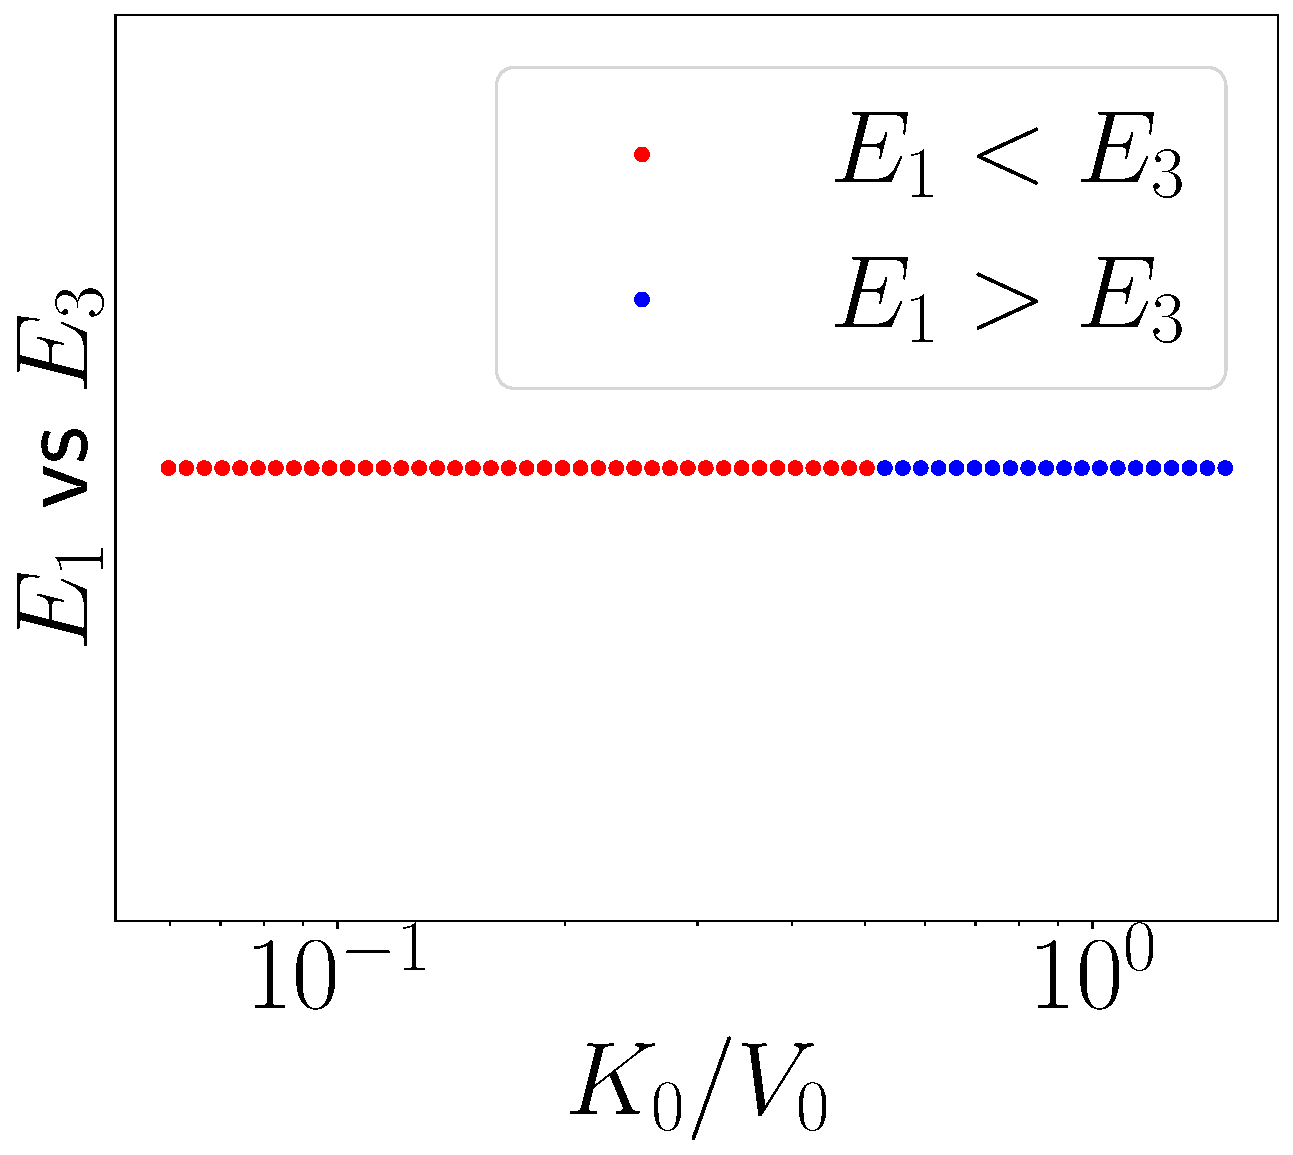
\includegraphics[width=0.5\textwidth]{../figures/E1_vs_E3.pdf}
\end{figure}

\subsection{Unscreened regime: \(-U_b/J > 1/4 \)}

\subsection{Approach towards the thermodynamic limit}

{\bf \Large [Update with V vs D plots]}

The URG method works strictly on finite systems and leads to finite values of fixed point couplings. The behaviour of the Hamiltonian in the thermodynamic limit can then be determined using finite-size scaling where we increase the bandwidth and decrease the width of each RG step. When applied to the fixed point value of the impurity-bath hybridisation parameter \(V\) (fig.~\ref{V_vs_D}), it can be seen that the fixed point value increases as the system size is increased, implying that the continuum limit of \(V^*\) is \(\infty\). This holds for both \(V_0 > J_0\) and \(V_0 < J_0\), as shown in the two panels of fig.~\ref{V_vs_D}.

\begin{figure}[!htb]
	\centering
	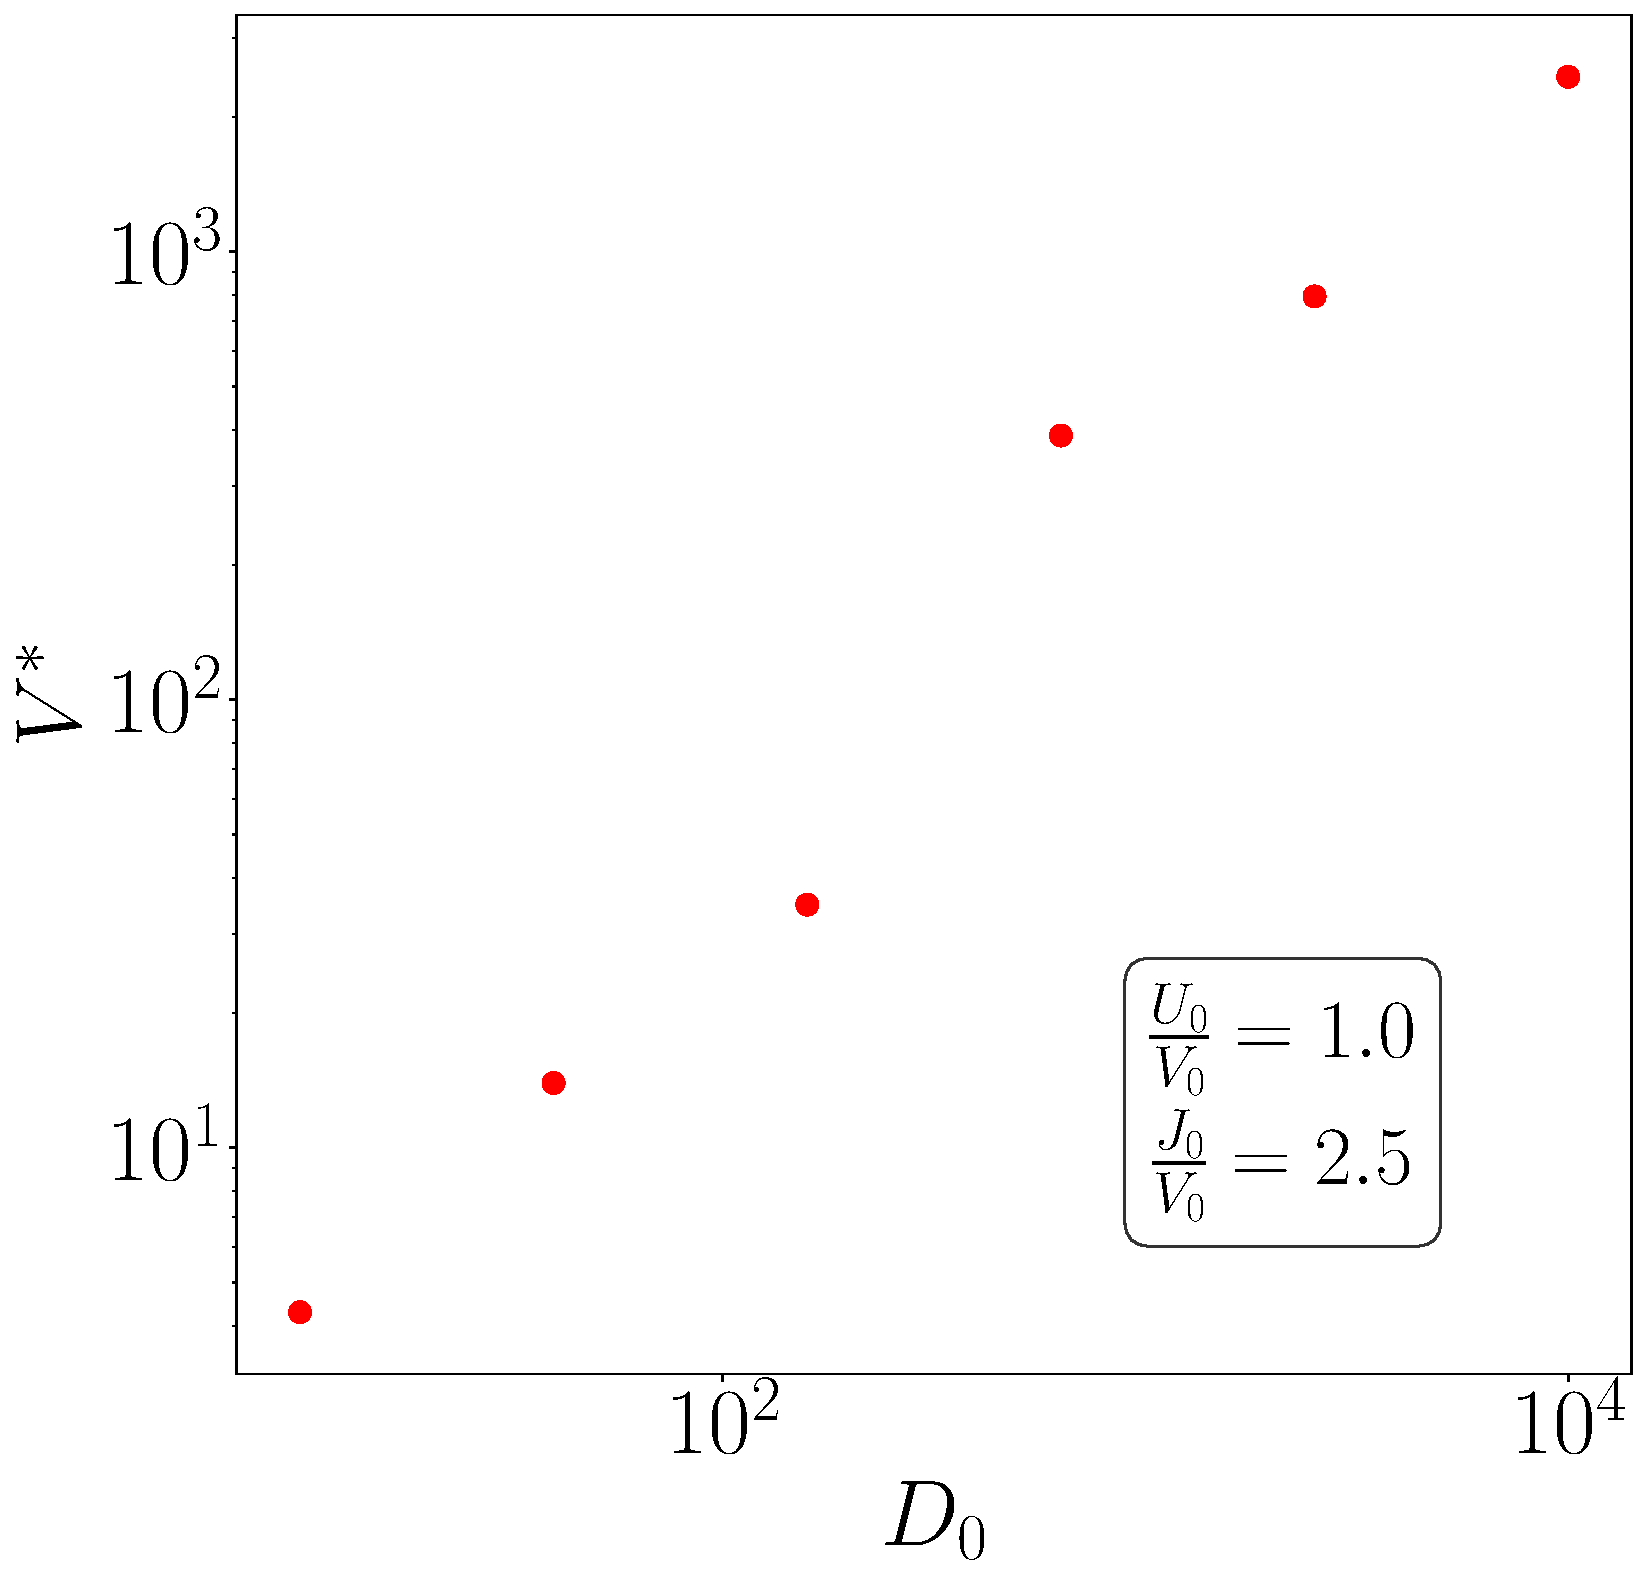
\includegraphics[width=0.4\textwidth]{../figures/Vstar_vs_D_smallV.pdf}
	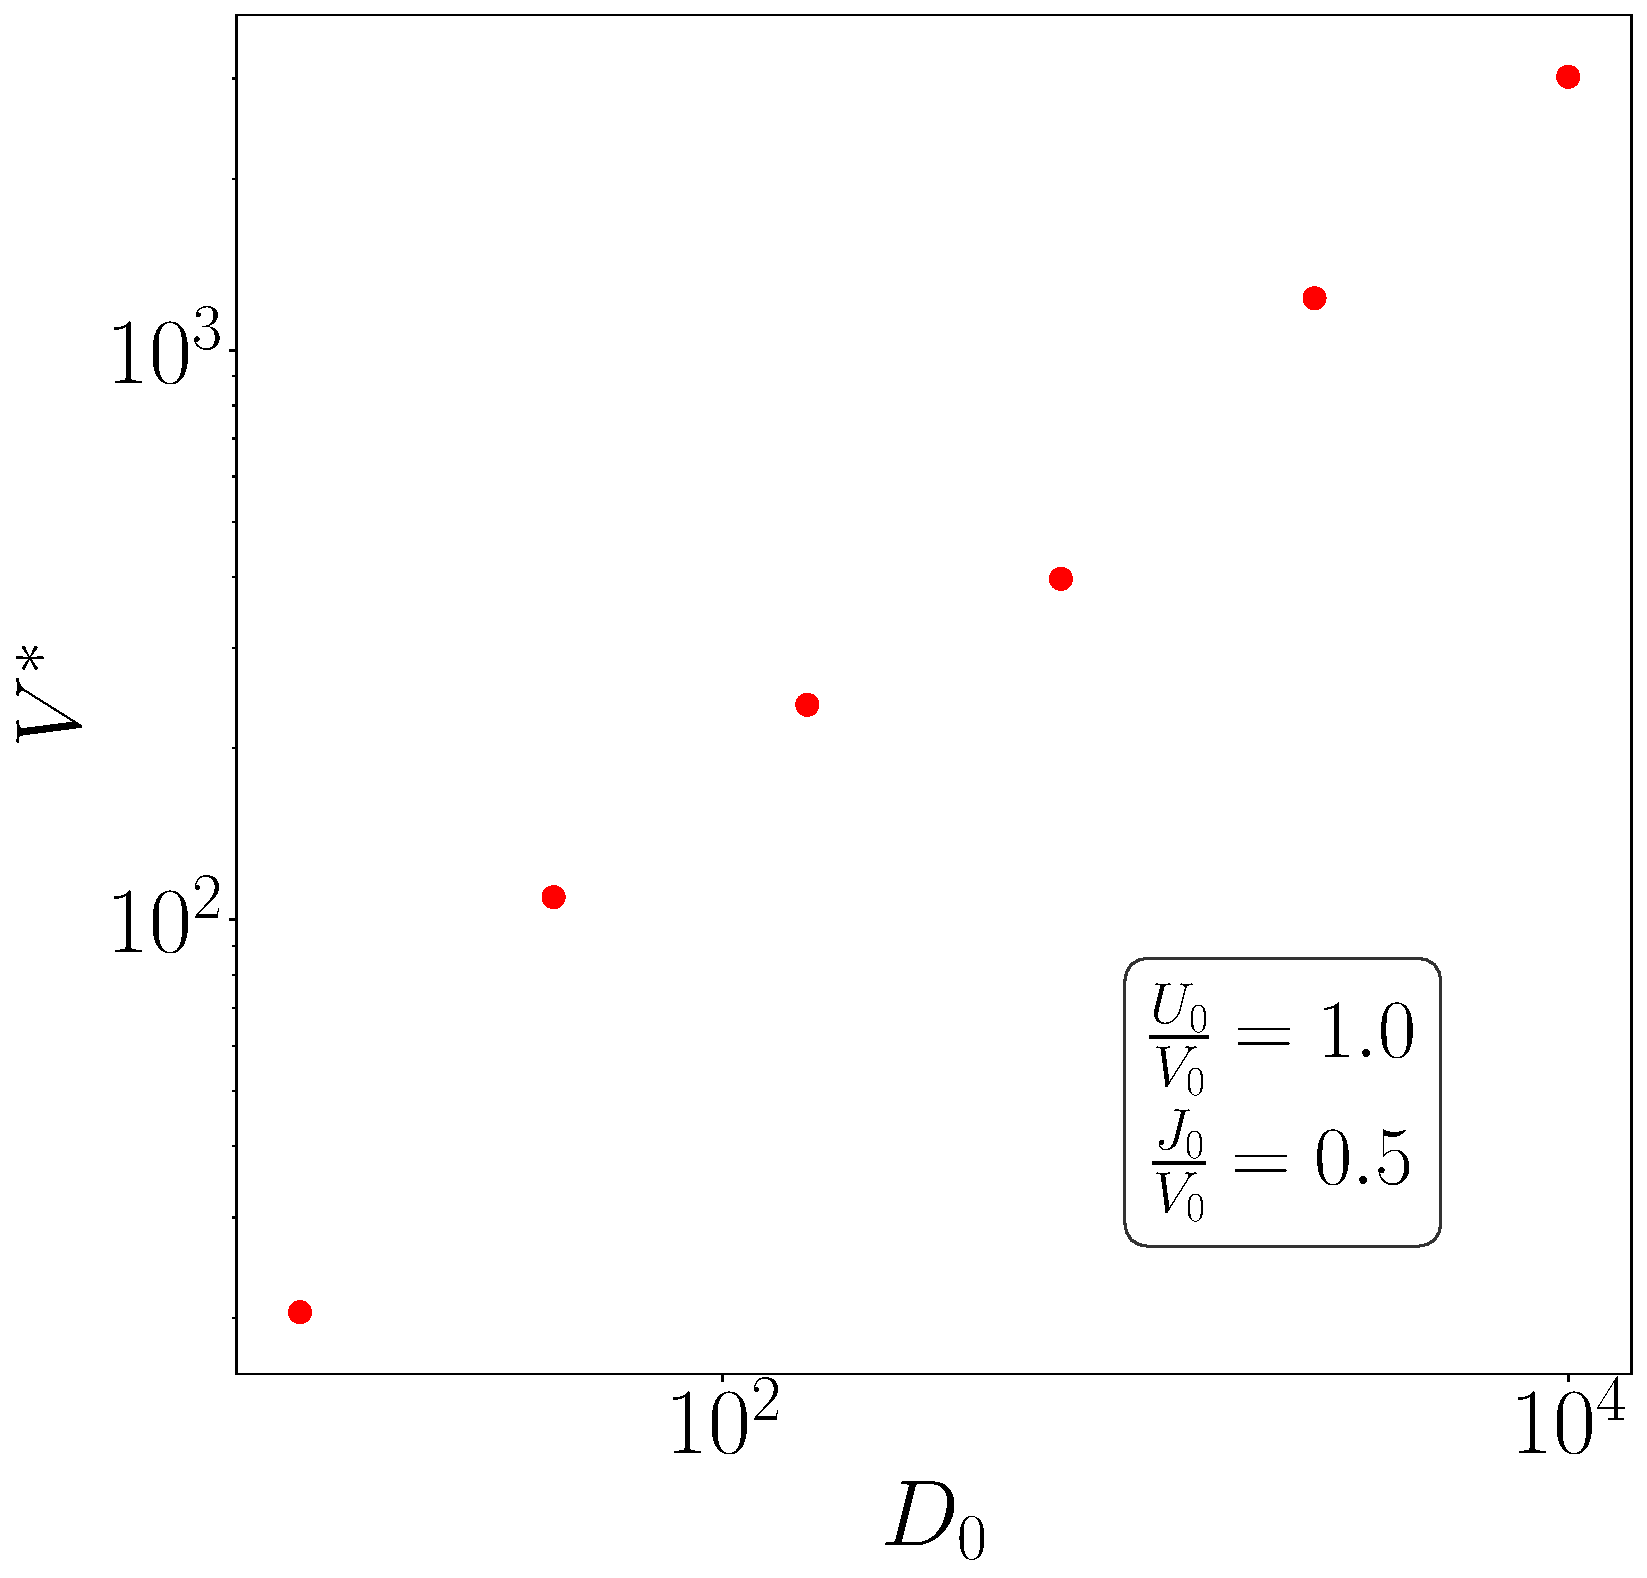
\includegraphics[width=0.4\textwidth]{../figures/Vstar_vs_D_largeV.pdf}
	\caption{Variation of fixed point value \(V^*\) with increasing bandwith \(D_0\), for both \(V_0 > J_0\) and \(V_0 < J_0\).}
	\label{V_vs_D}
\end{figure}

In a similar manner, we checked the variation of the spin and charge probabilities, \(c_s\) and \(c_c\), in the ground state, with increasing bandwith. The result is shown in fig.~\ref{c_vs_D}.
\begin{figure}[!htb]
	\centering
	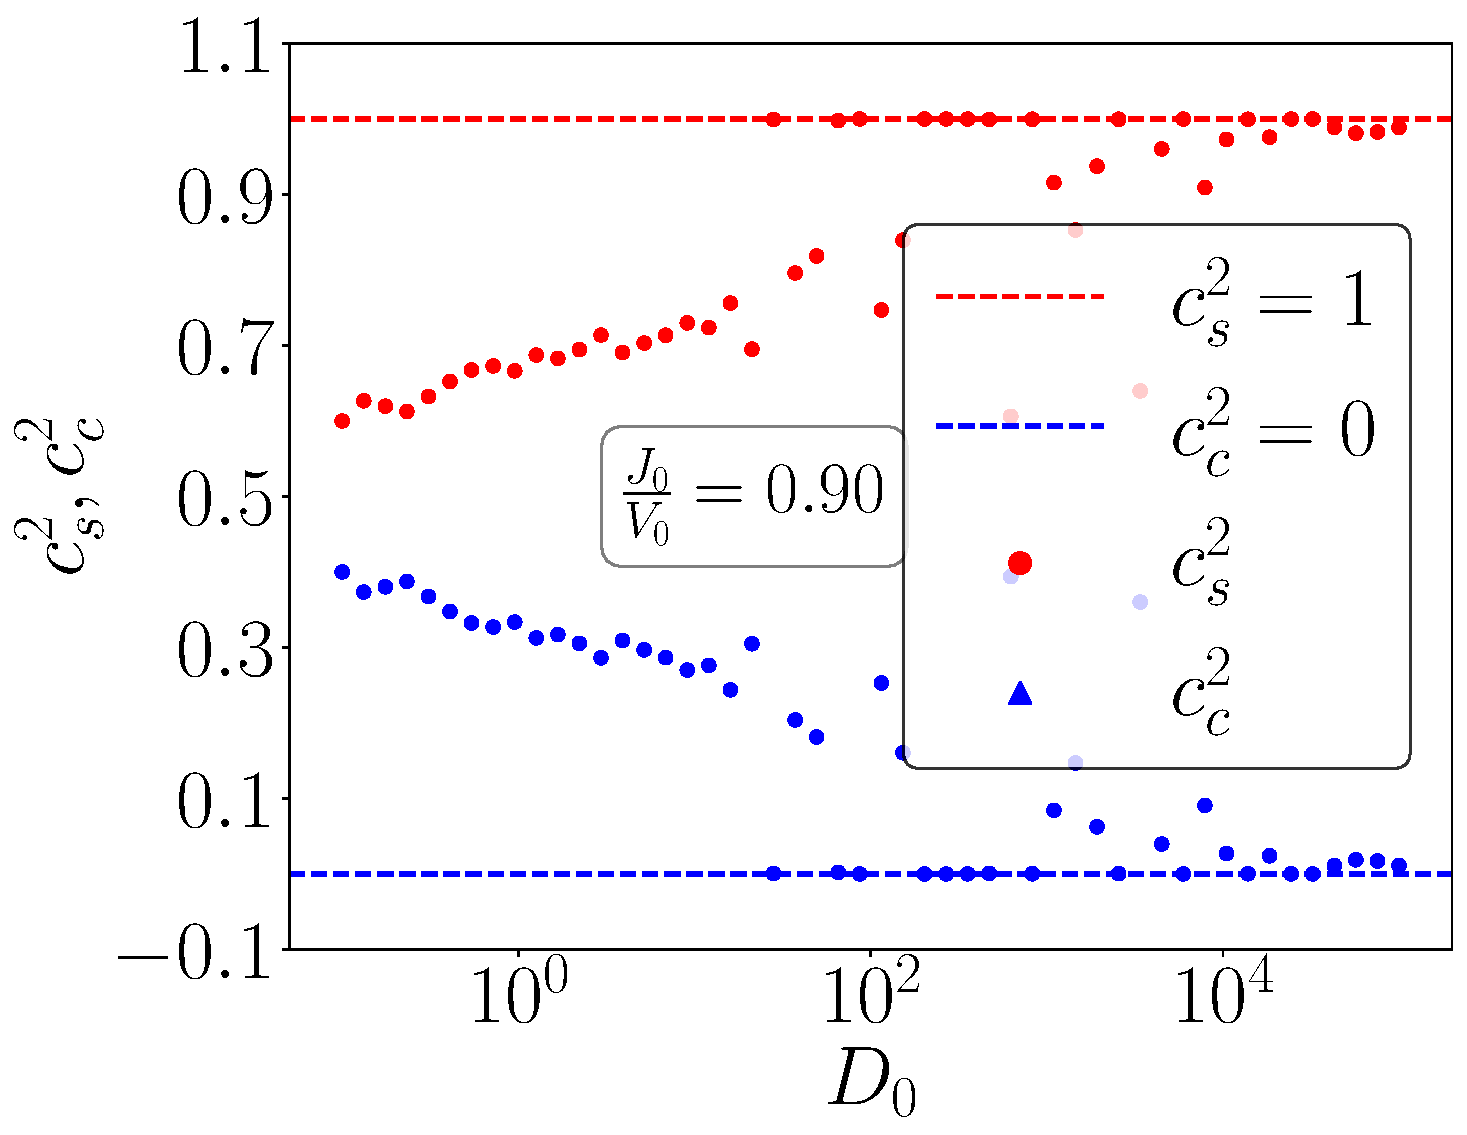
\includegraphics[width=0.45\textwidth]{../figures/coeffs_vs_D.pdf}
	\caption{Variation of spin and charge fractions, \(c_s\) and \(c_c\), of the ground state, as a function of bare bandwidth \(D_0\). Left and right panels show the cases of \(J_0 < V_0\) and \(J_0 > V_0\) respectively.}
	\label{c_vs_D}
\end{figure}
For both \(V_0 < J_0\) and \(V_0 > J_0\), we see that the spin contribution increases towards unity while the charge contribution vanishes. This indicates that at large bandwidth, the ground state becomes purely a spin singlet, formed purely by singly-occupied impurity states.
\begin{equation}\begin{aligned}
	\label{gstate_kondo}
	\lim_{D_0 \to \infty} \ket{\Psi}_1 = \frac{1}{\sqrt 2}\left(\ket{\uparrow, \downarrow} - \ket{\downarrow, \uparrow}\right) 
\end{aligned}\end{equation}

\subsection{The critical point: \(-U_b/J = 1/4 \)}

\section{Evolution of the groundstate across the transition}

\subsection*{Overlap of ground state against spin singlet and charge triplet zero states}

\begin{figure}
	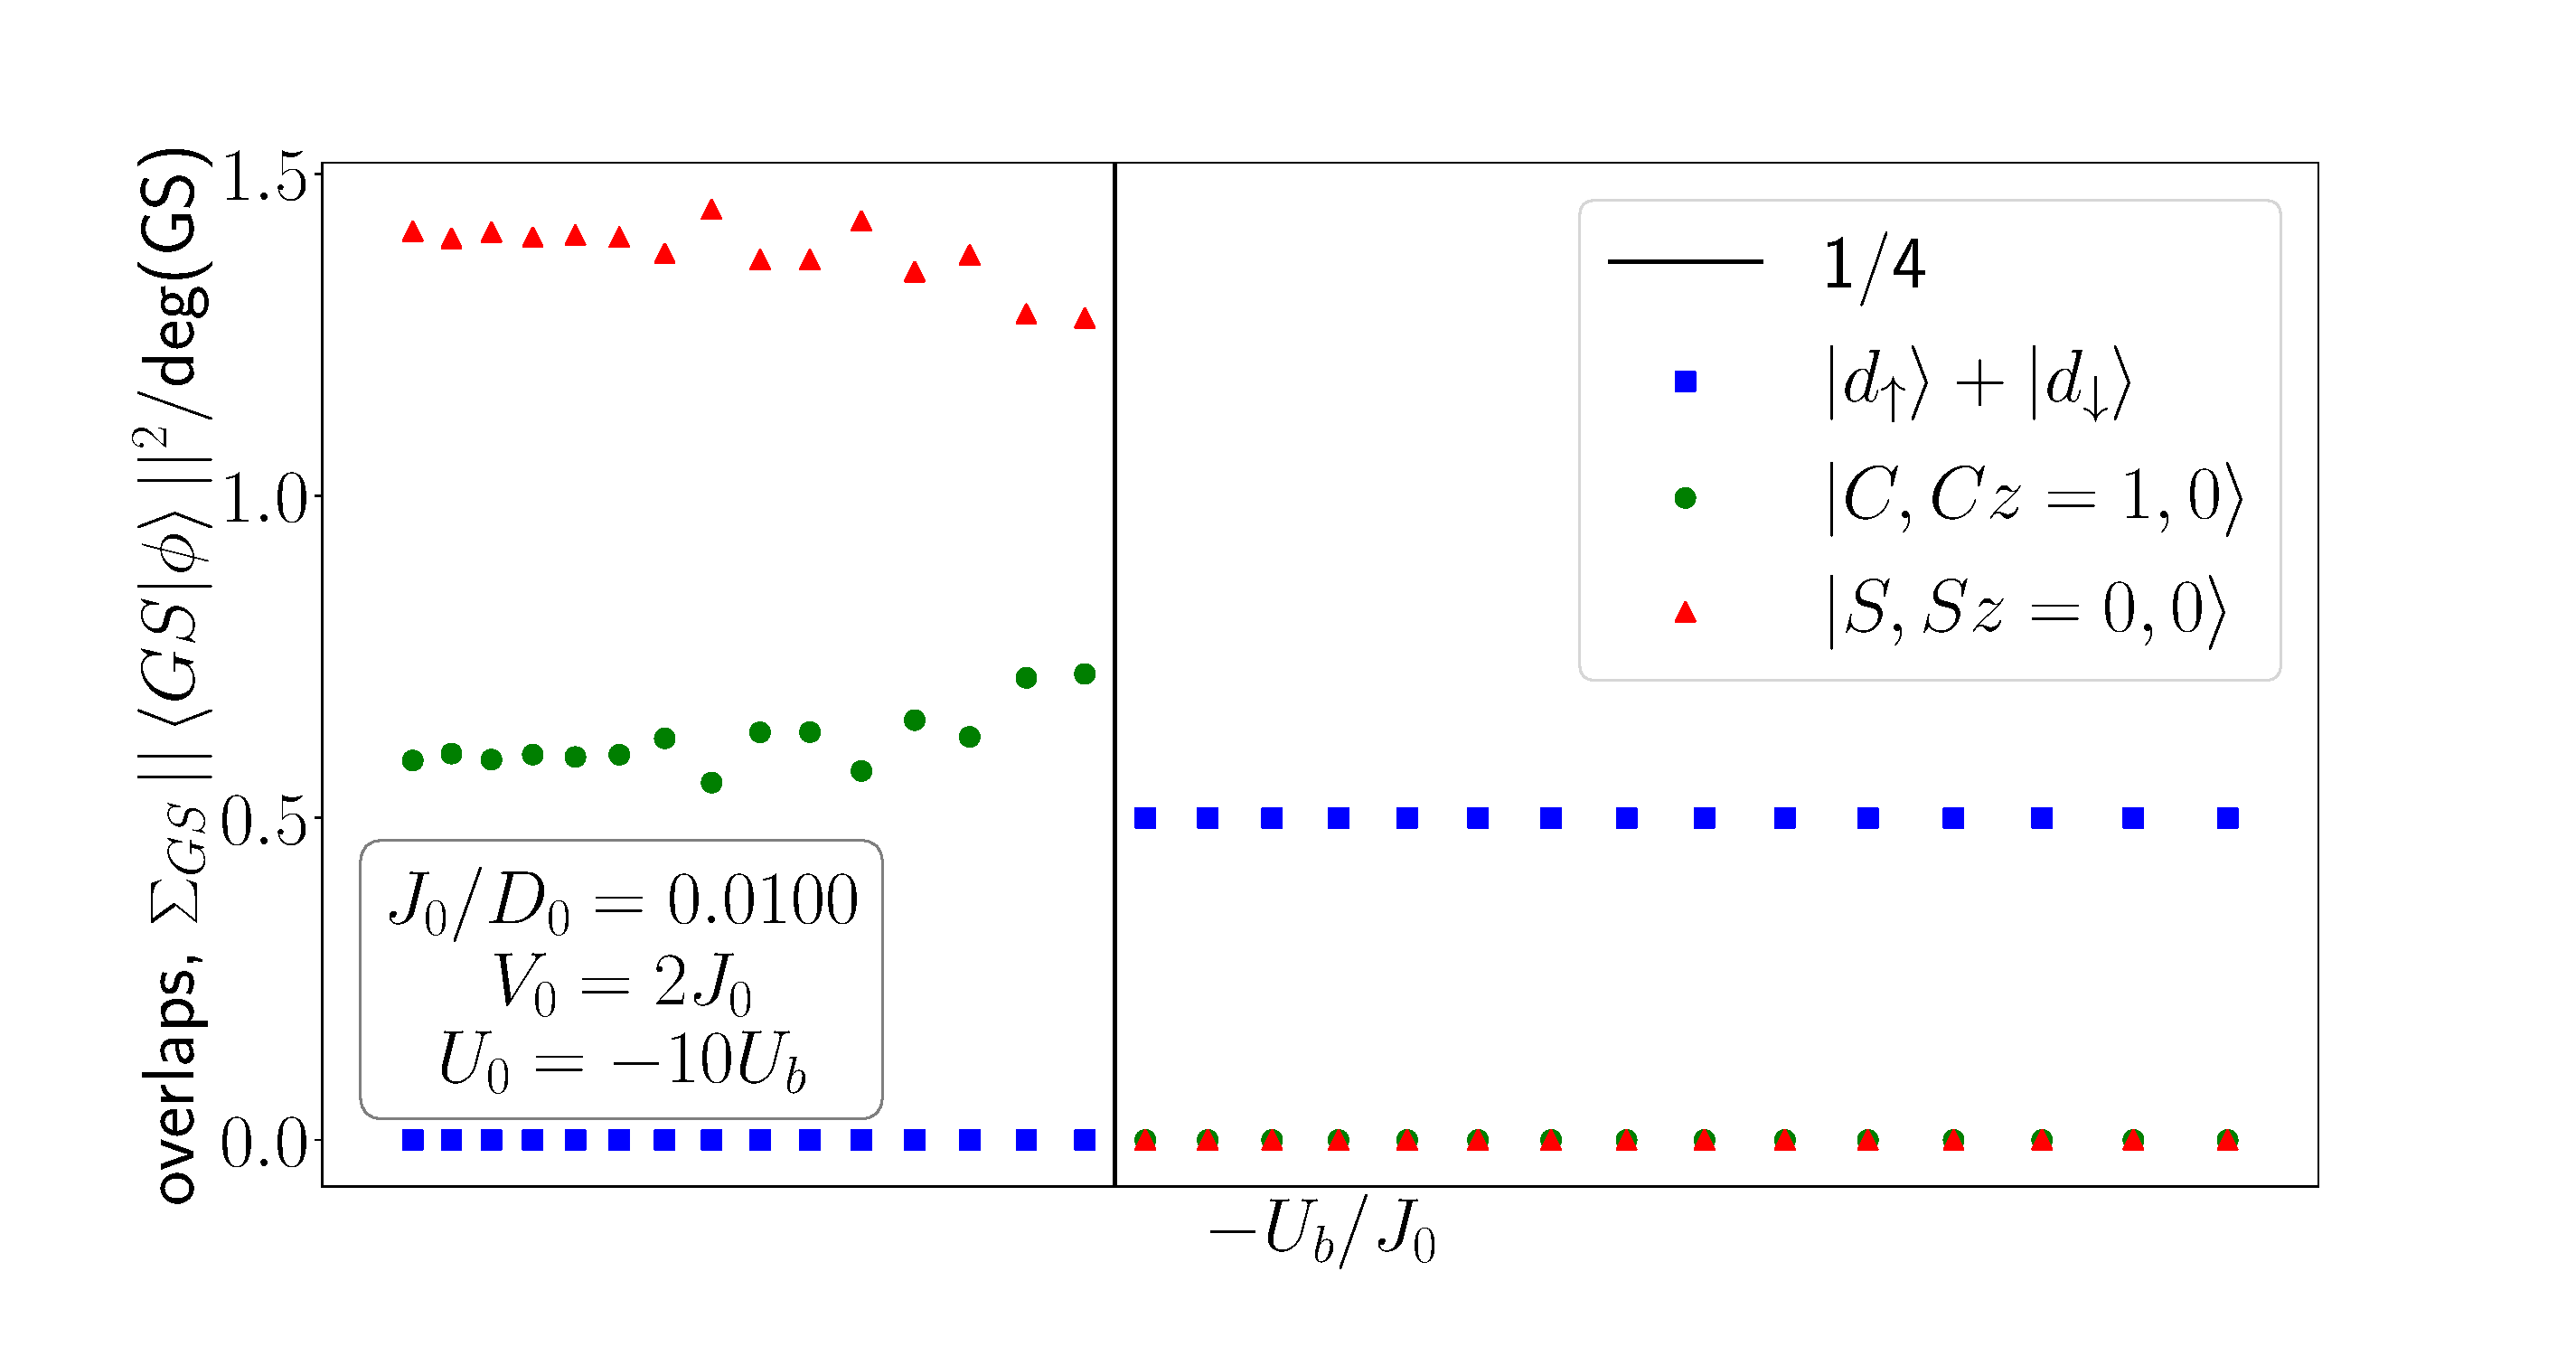
\includegraphics[width=0.5\textwidth]{../figures/overlaps_gs-J=10.000.pdf}\\
	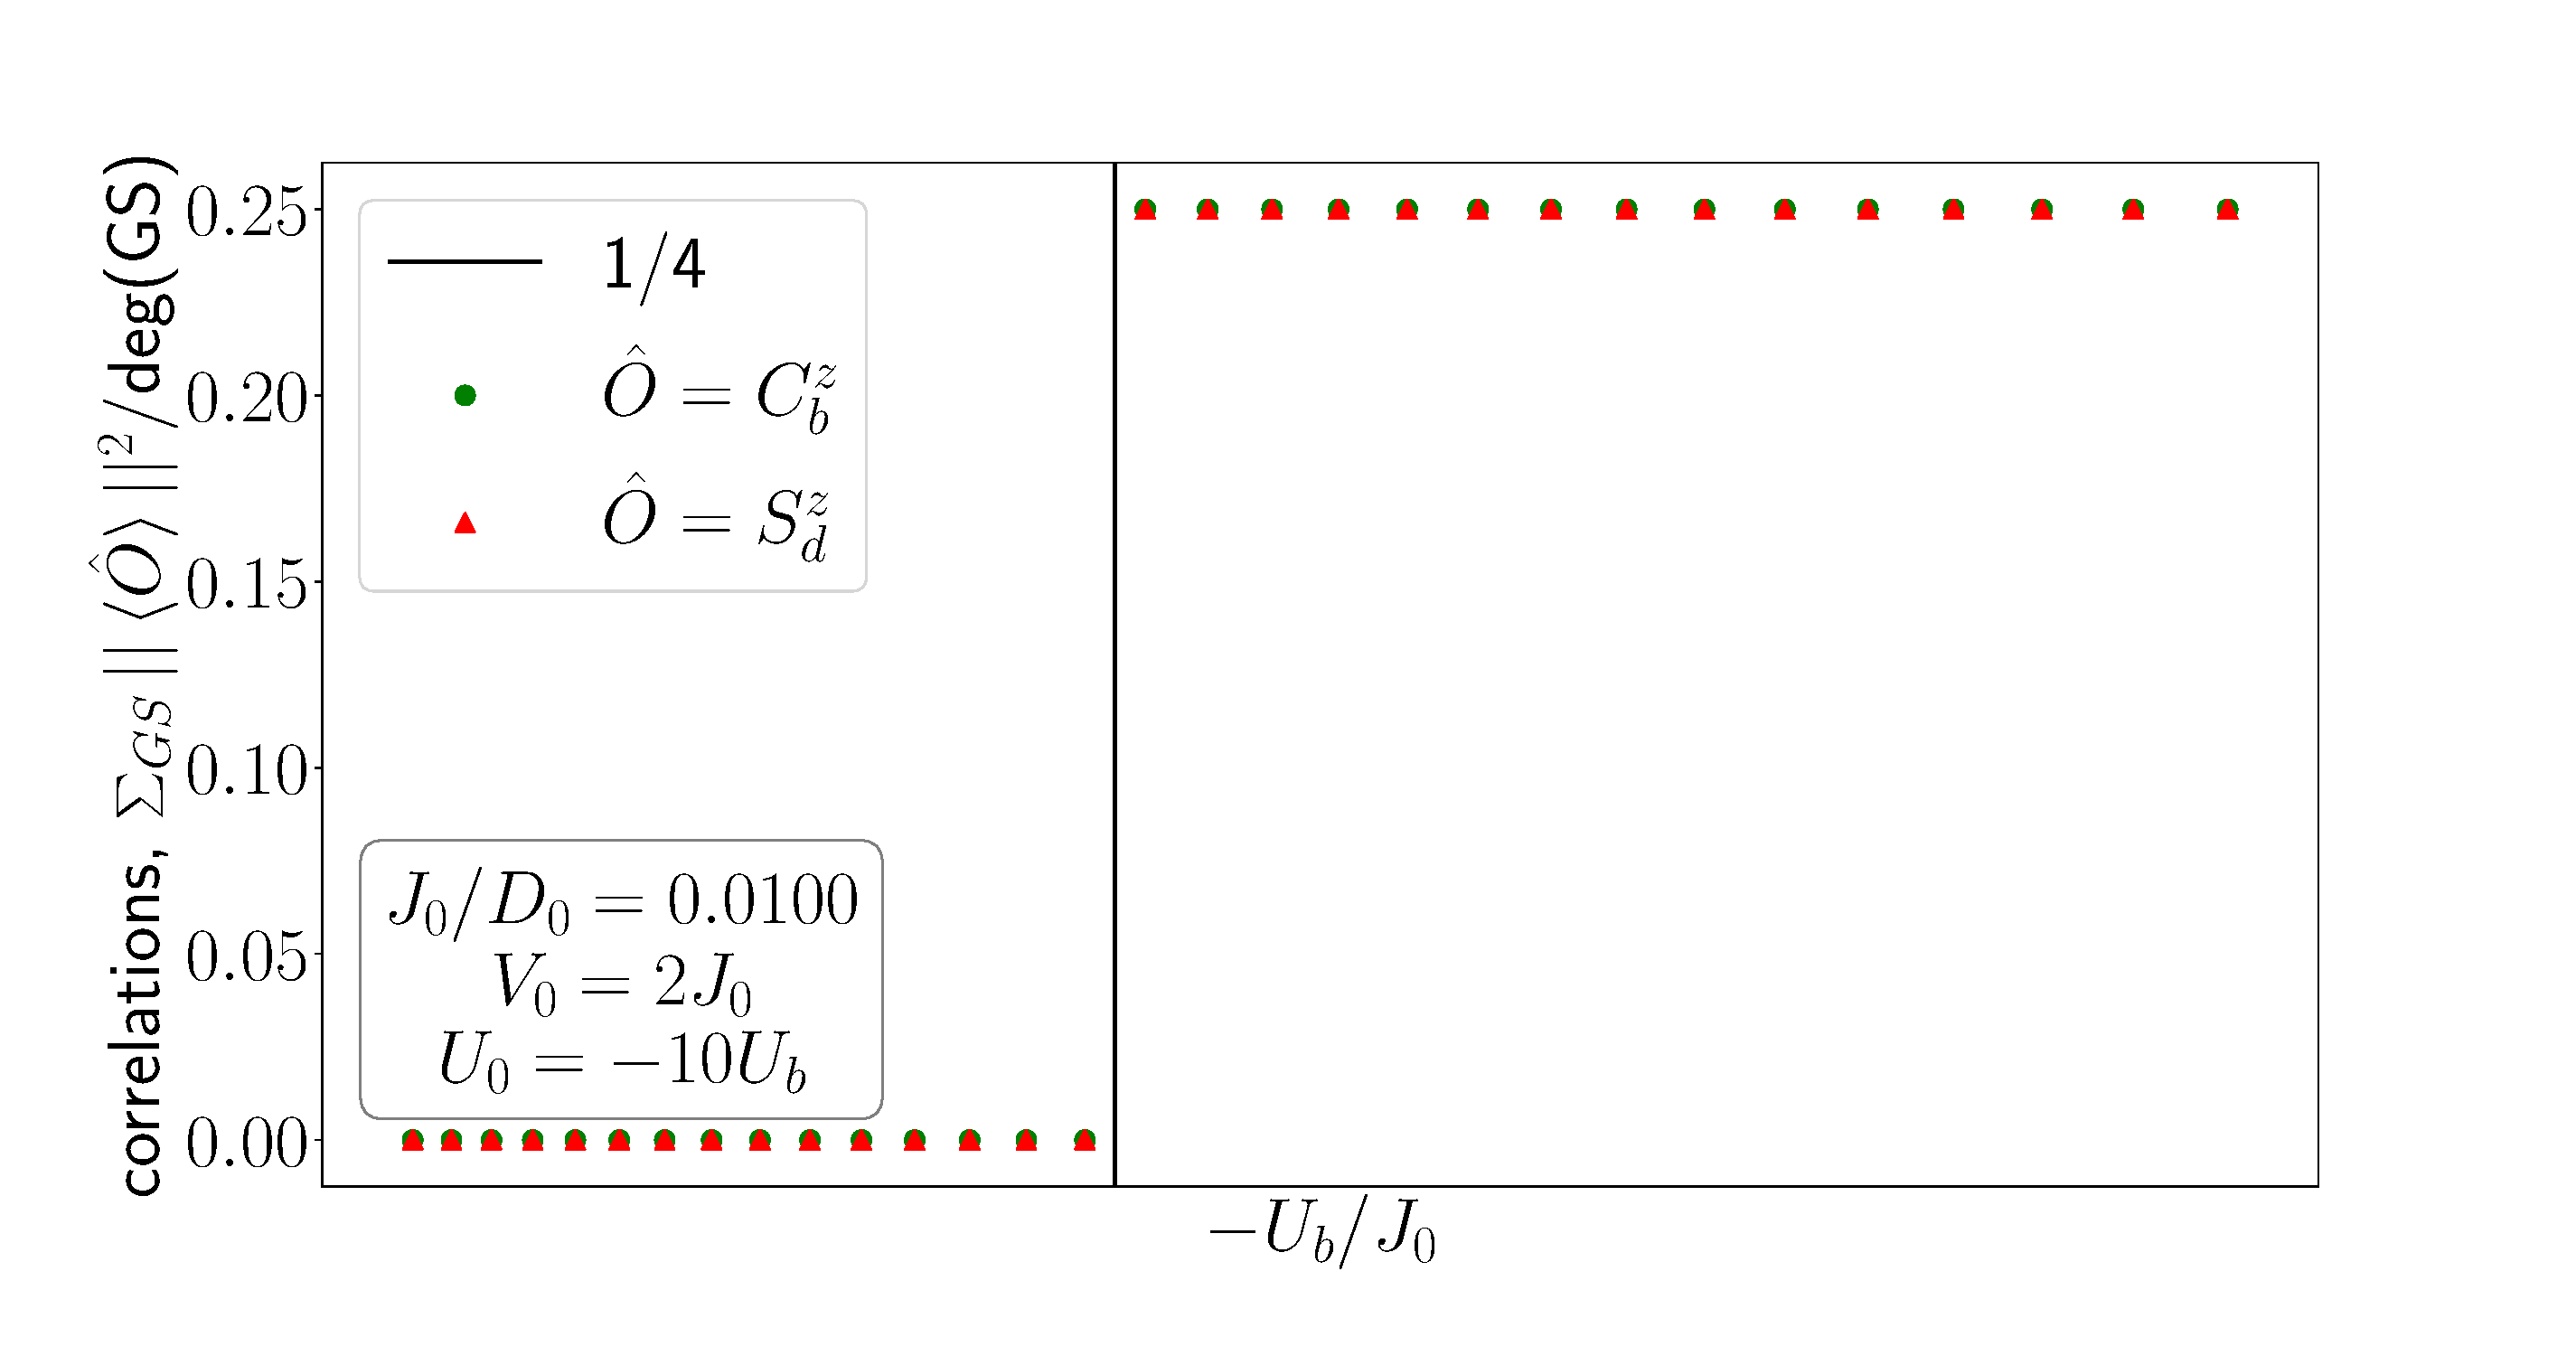
\includegraphics[width=0.5\textwidth]{../figures/corrs_gs-J=10.000.pdf}
\end{figure}


\subsection{Presence of sub-dominant pair fluctuations}

\begin{figure}
	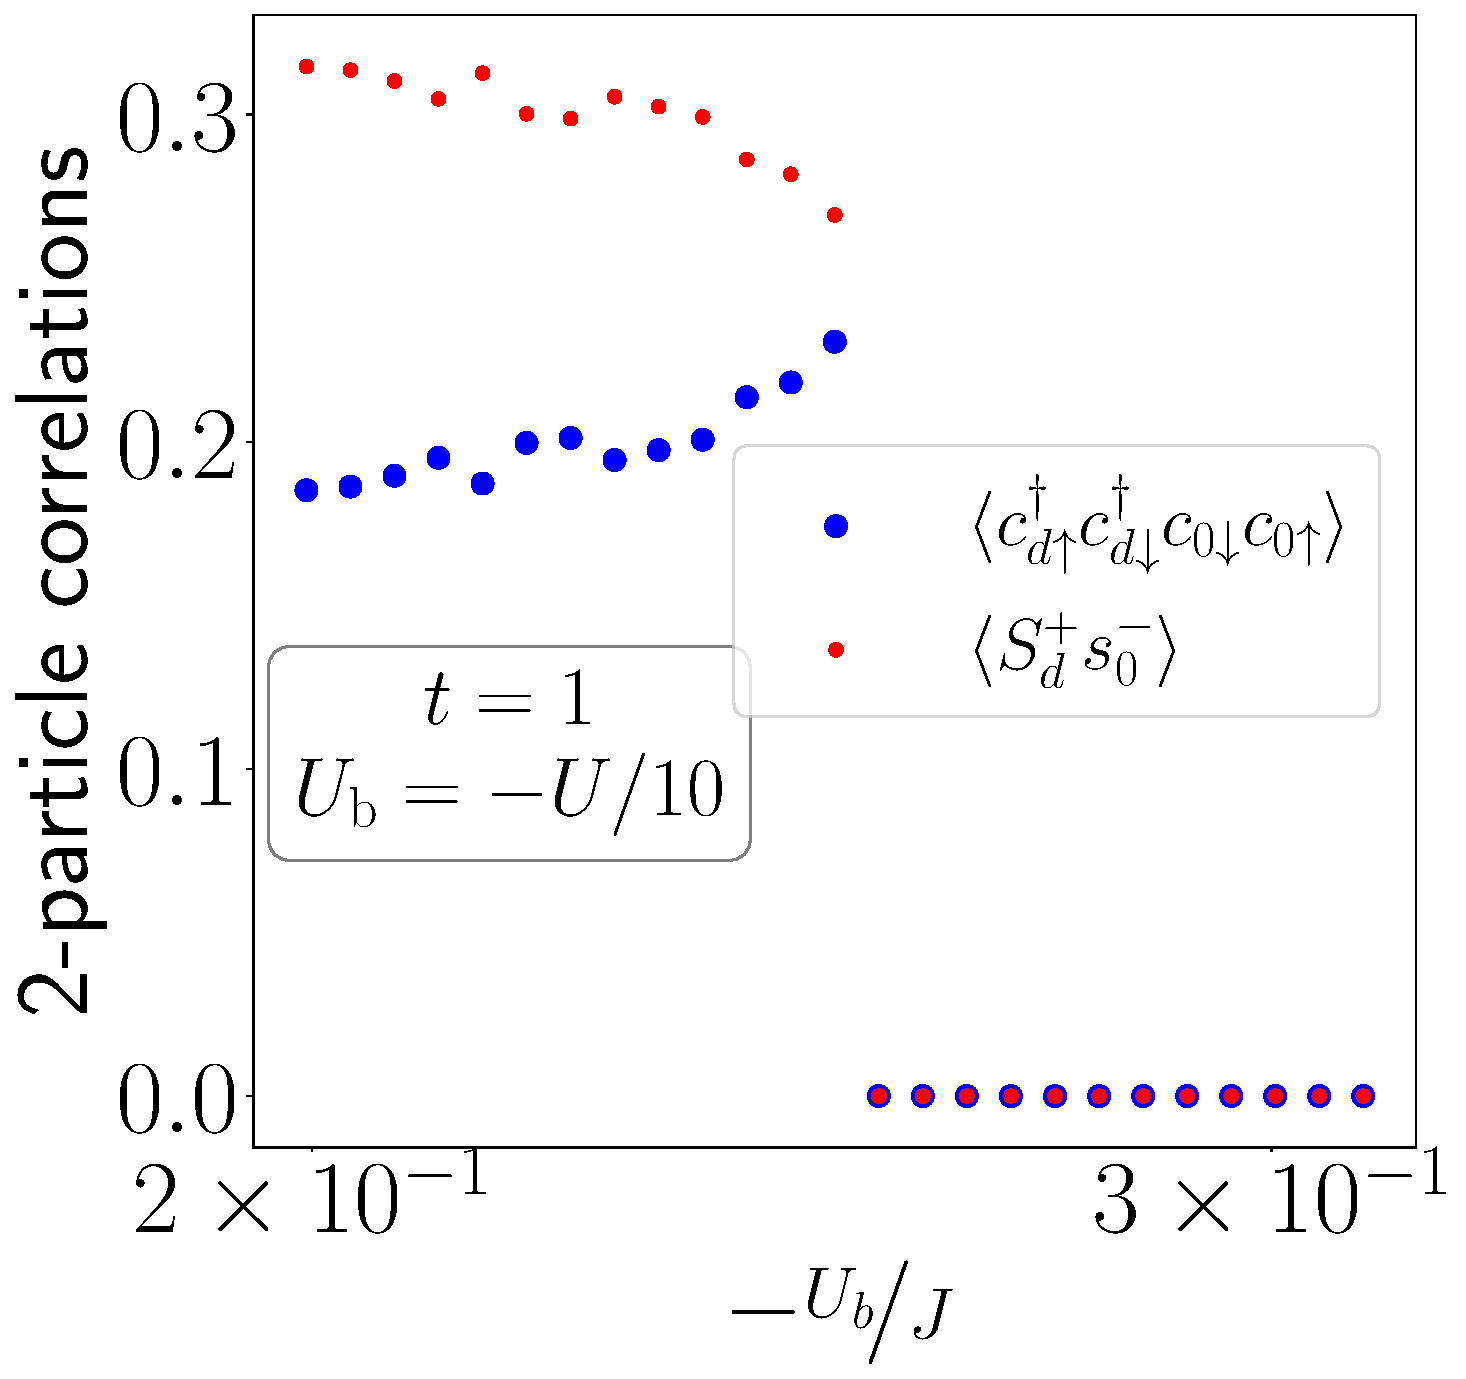
\includegraphics[width=0.4\textwidth]{../figures/odlro-D=1000.00000,t=1.00000,J=30.00000,V=1.50000J,Ub=-Uby10,N=4,U=59.85787,93.55363,25.pdf}
	\caption{Growth of pair fluctuations \(p^\dagger_d p_0\) between the impurity and the zeroth site towards the critical point, \(p^\dagger=c^\dagger_\uparrow c^\dagger_\downarrow\) being the local pair creation operator. This comes at the cost of the spin-flip fluctuations \(S_d^+ s_0^- + \text{h.c.}\). which decrease towards the transition.}
	\label{pair_fluc}
\end{figure}

The behaviour of the various kinds of correlation functions (for eg., the reduction of the impurity compensation \(\vec{S}_d\cdot\vec{s}_0\)) shown above indicate that the Kondo cloud that screens the impurity is getting destroyed as \(U_b/J\) increases in magnitude. To shed some light on the nature of the fluctuations that faciliate this process, we also plot the average pair fluctuation in the ground state as a function of \(U_b/J\), in fig.~\ref{pair_fluc}. The pair fluctuations are terms that transfer an electron pair between the impurity and zeroth sites: \(c^\dagger_{d \uparrow}c^\dagger_{d \downarrow} c_{0 \downarrow}c_{0 \uparrow}\). It can be seen from the figure that while the spin-flip fluctuations decrease (since the Kondo cloud is formed out of these spin-flip fluctuations, this is consistent with the destruction of the Kondo cloud discussed in this paragraph), the pair fluctuations pick up. Since the spin subspace and charge subspace cannot coincide on the same site, we can then conclude that it is the growth of these pair fluctuations brought about by the presence of the purely local interaction \(U_b\) that make the screening of the impurity spin very poor.

\subsection*{Correlations in ground state}
\begin{figure*}
	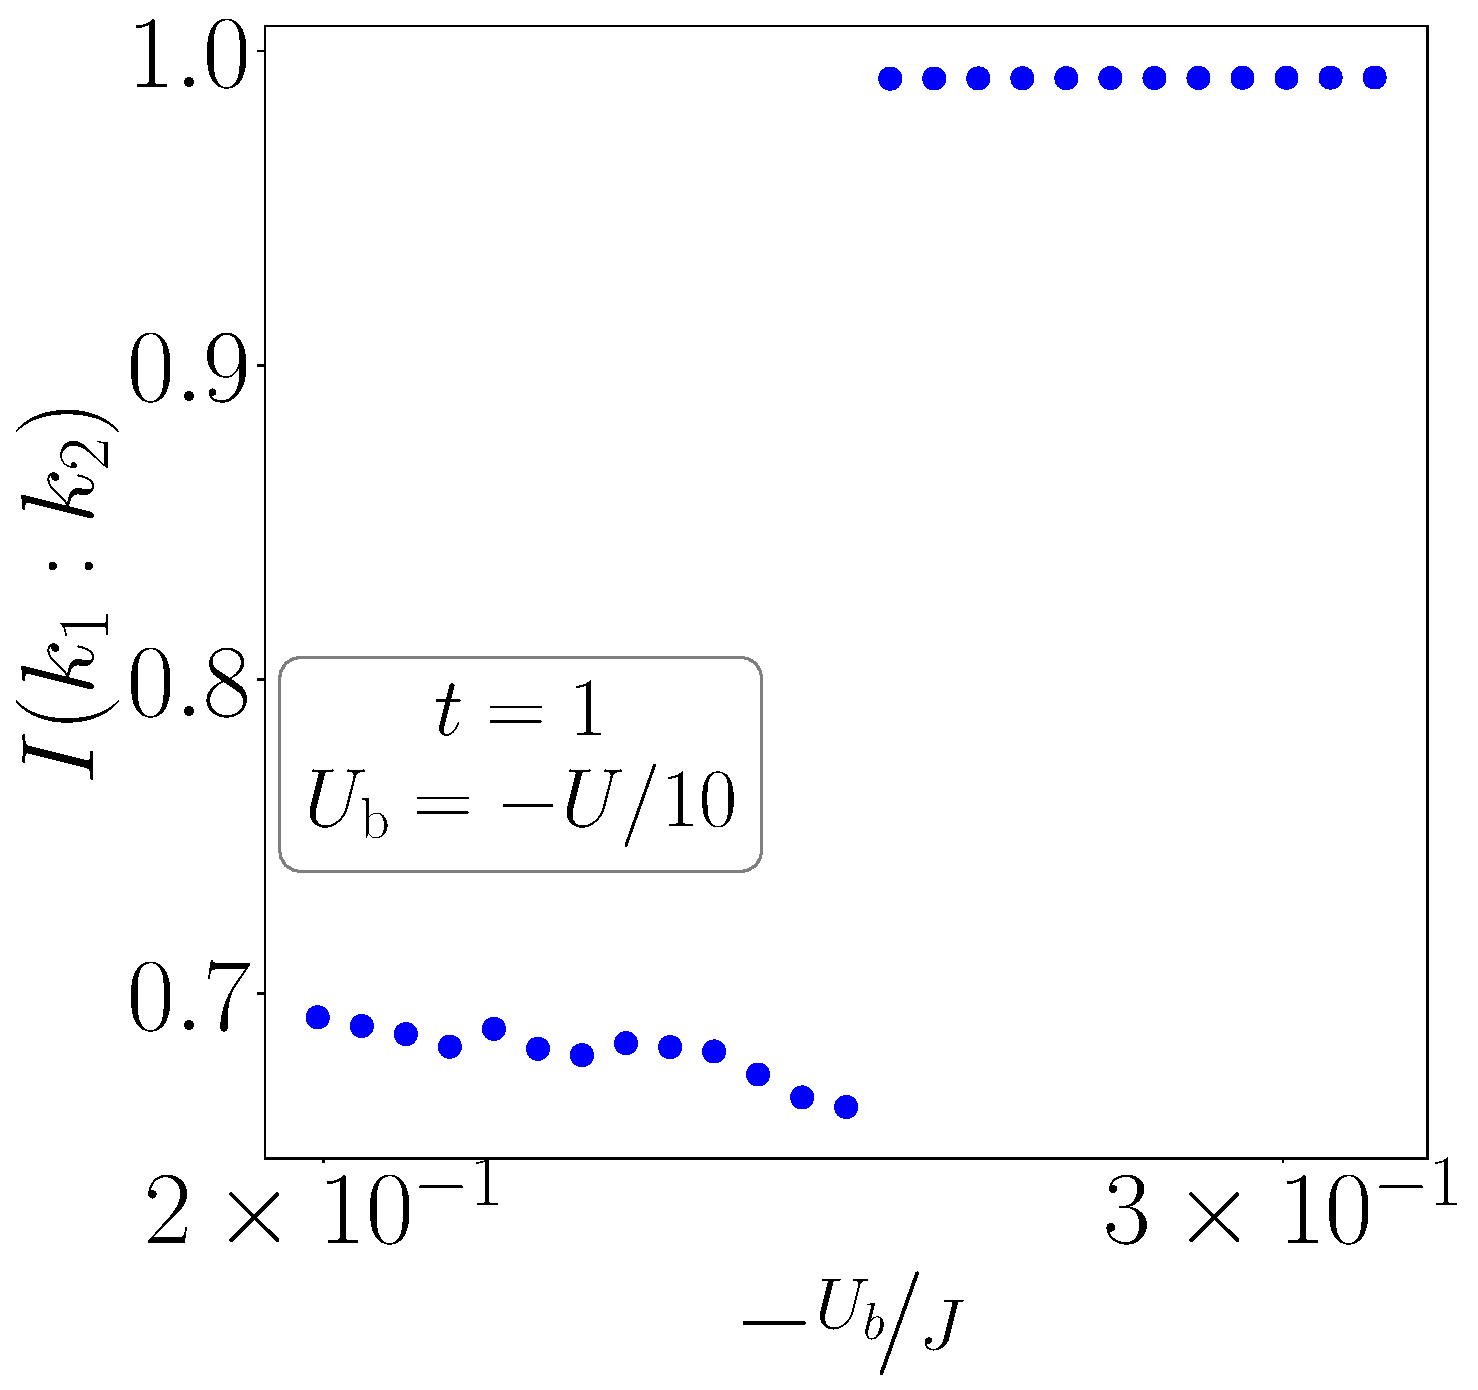
\includegraphics[width=0.45\textwidth]{../figures/corr-k-D=1000.00000,t=1.00000,J=30.00000,V=1.50000J,Ub=-Uby10,N=4,U=59.85787,93.55363,25.pdf}
	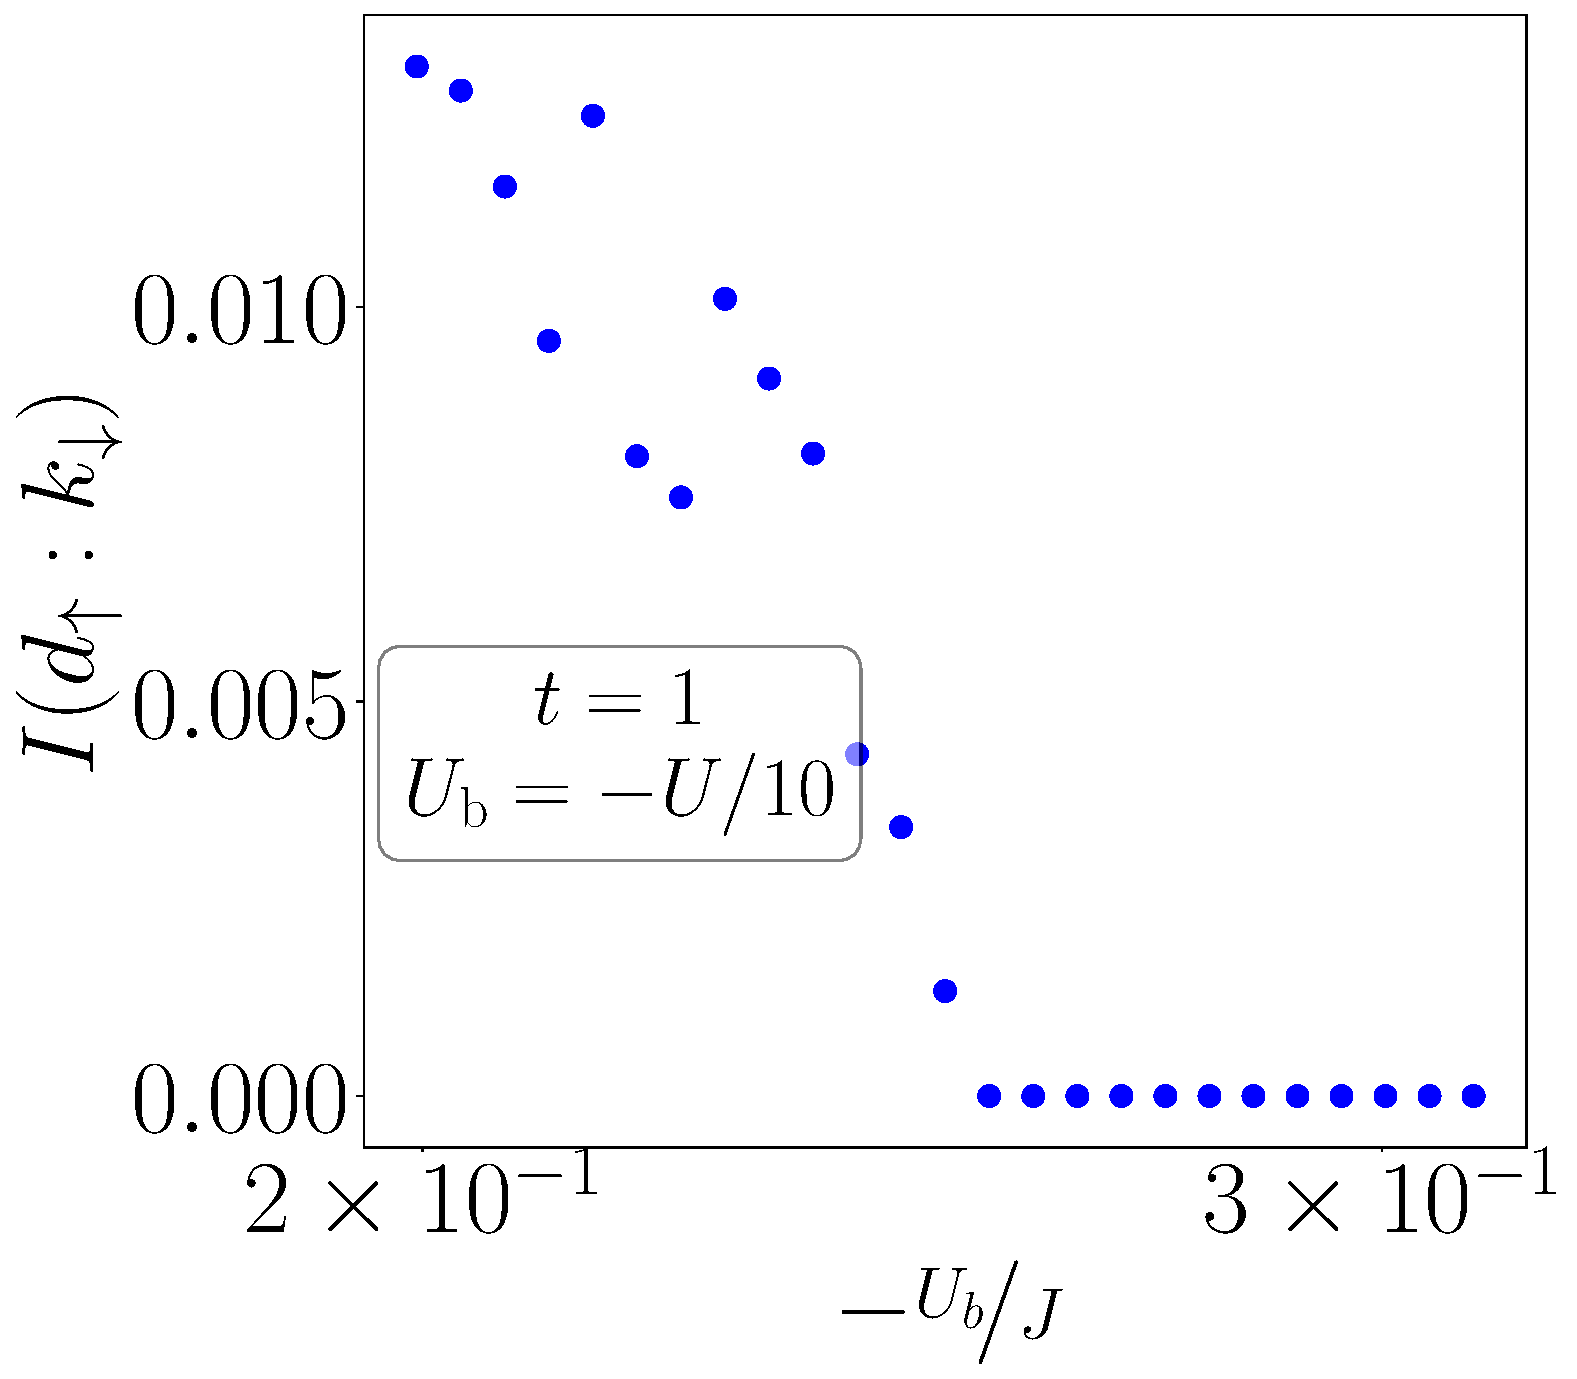
\includegraphics[width=0.45\textwidth]{../figures/mi-dk-D=1000.00000,t=1.00000,J=30.00000,V=1.50000J,Ub=-Uby10,N=4,U=59.85787,93.55363,25.pdf}
	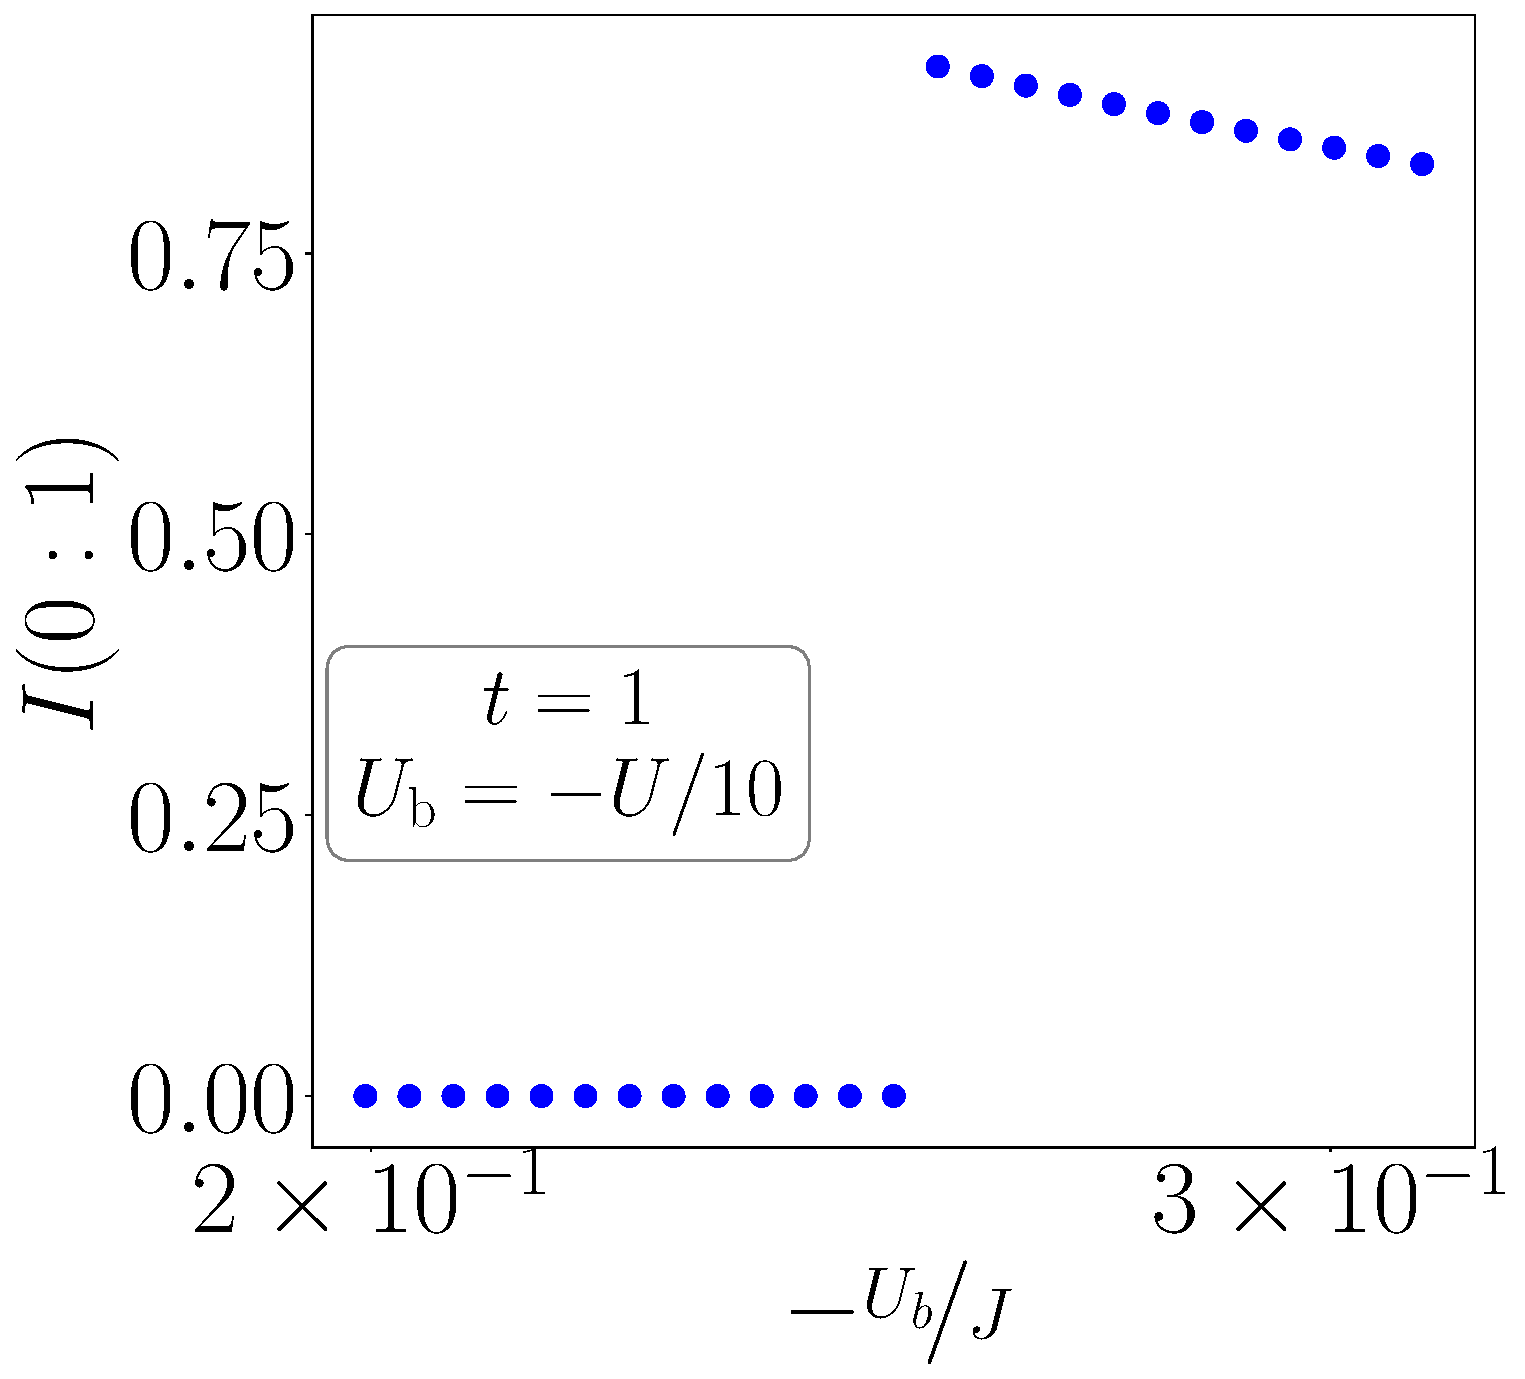
\includegraphics[width=0.45\textwidth]{../figures/mi-01-D=1000.00000,t=1.00000,J=30.00000,V=1.50000J,Ub=-Uby10,N=4,U=59.85787,93.55363,25.pdf}
	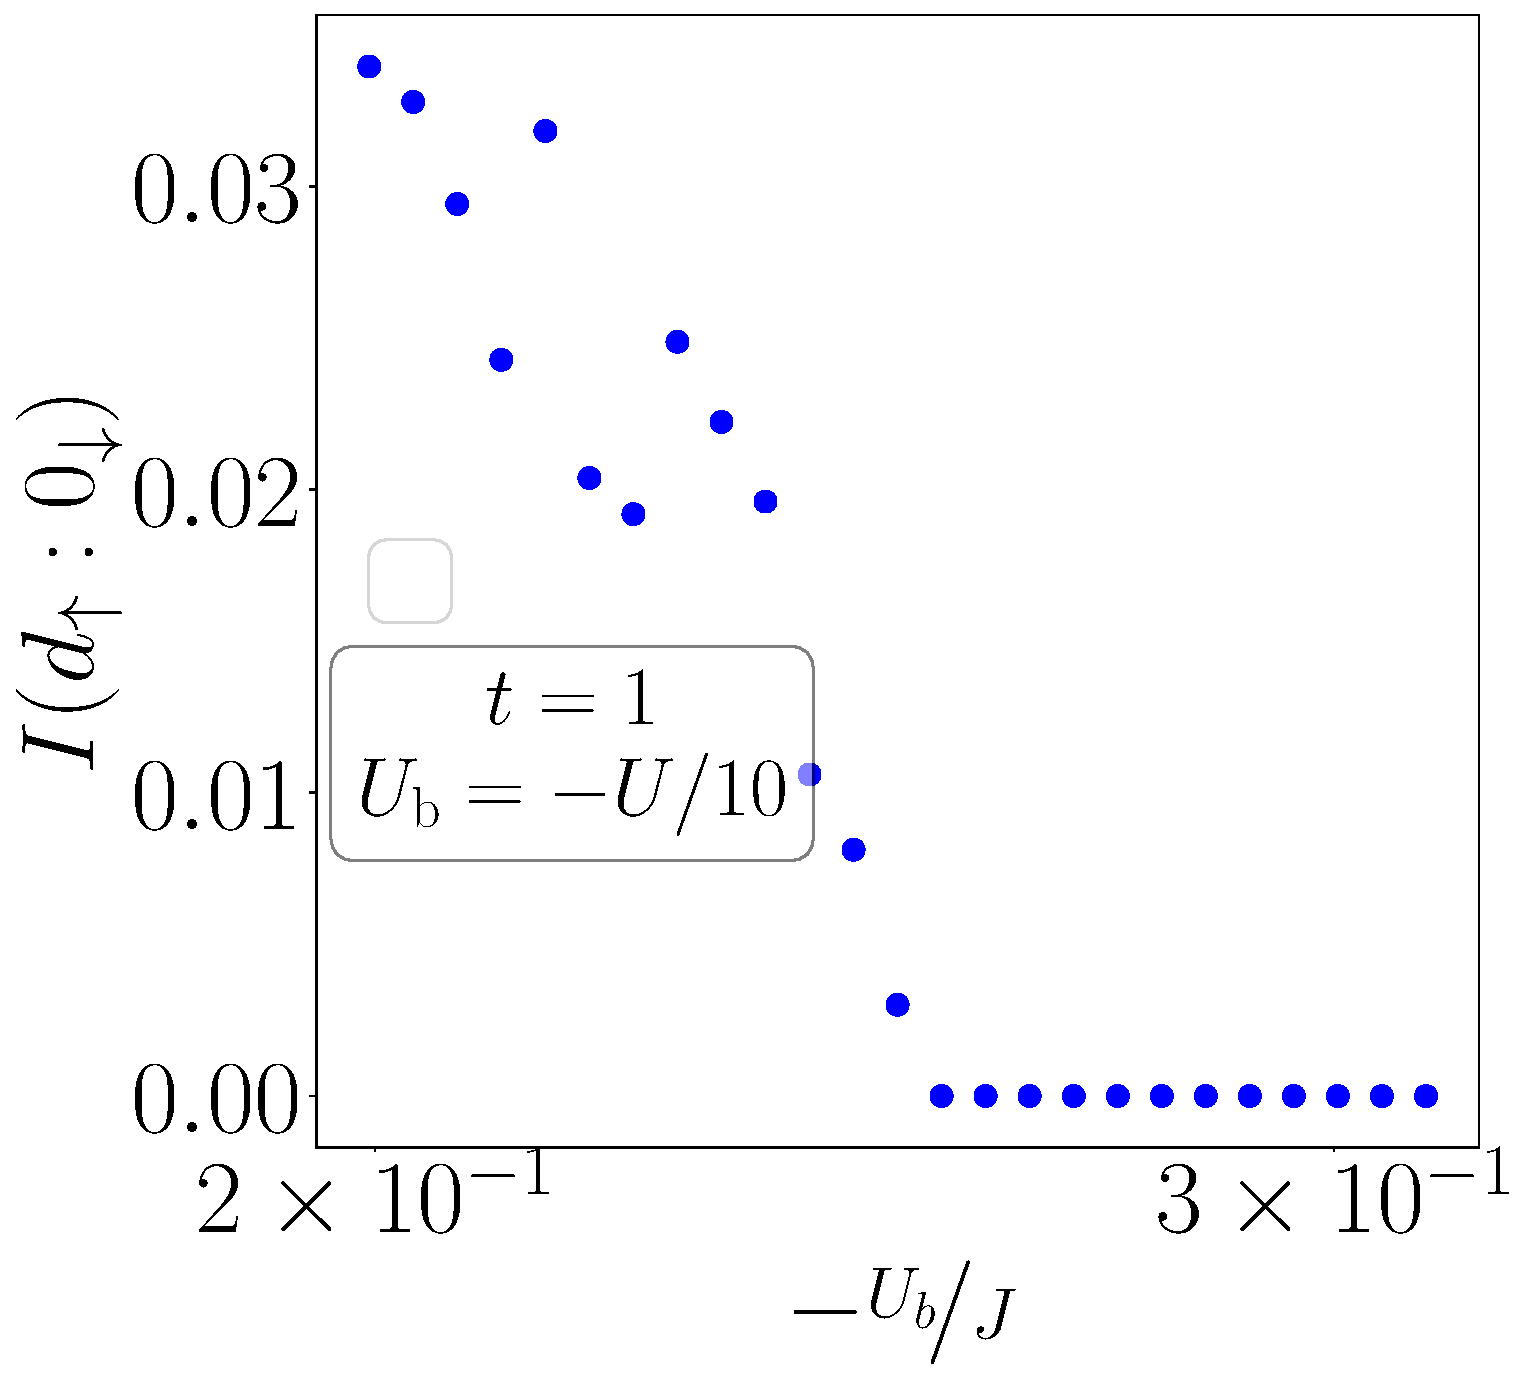
\includegraphics[width=0.45\textwidth]{../figures/mi-d0-D=1000.00000,t=1.00000,J=30.00000,V=1.50000J,Ub=-Uby10,N=4,U=59.85787,93.55363,25.pdf}
	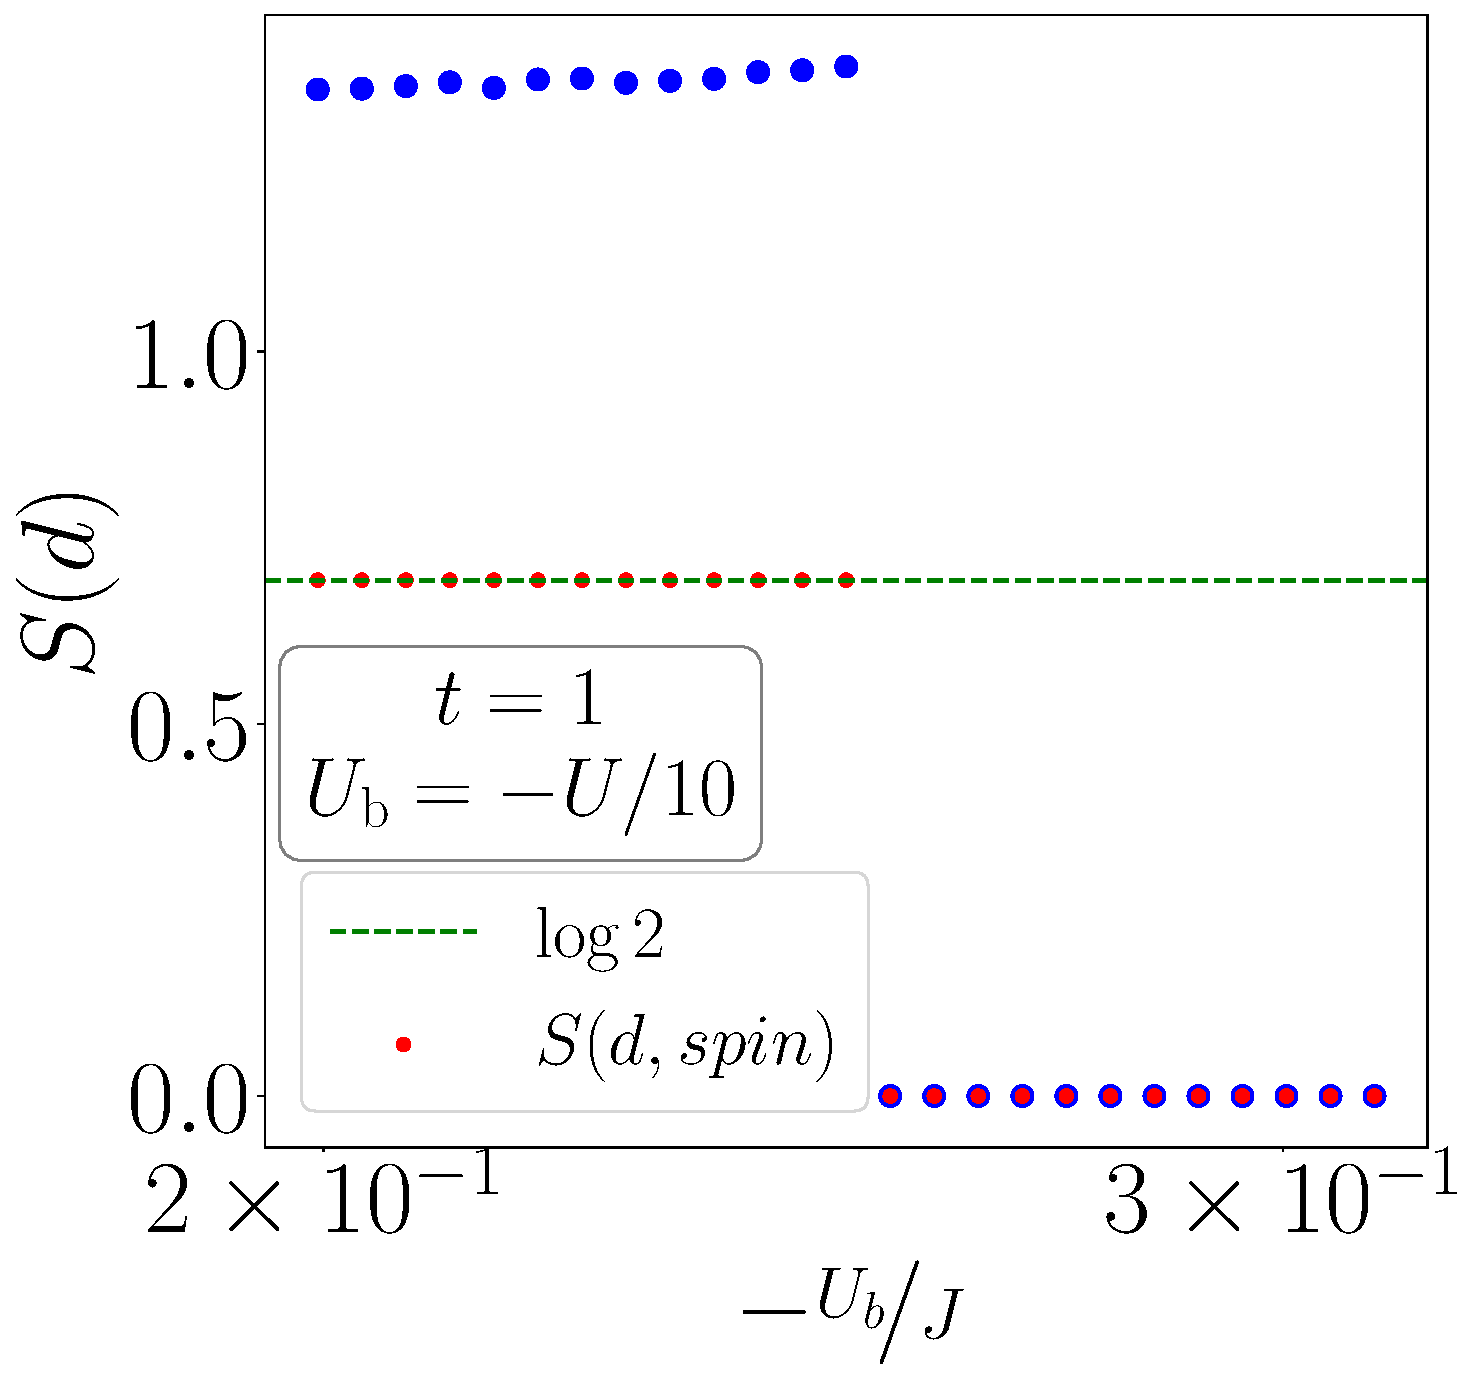
\includegraphics[width=0.45\textwidth]{../figures/EE-d-D=1000.00000,t=1.00000,J=30.00000,V=1.50000J,Ub=-Uby10,N=4,U=59.85787,93.55363,25.pdf}
\end{figure*}


\subsection{Impurity spectral function \(A_{dd}(\omega)\)}
These are the frequency-domain spectral functions for the retarded propagator \(-i\theta(t)\left<\left\{c_{d\sigma}(t),c^\dagger_{d\sigma}\right\}  \right>\):
\begin{center}
	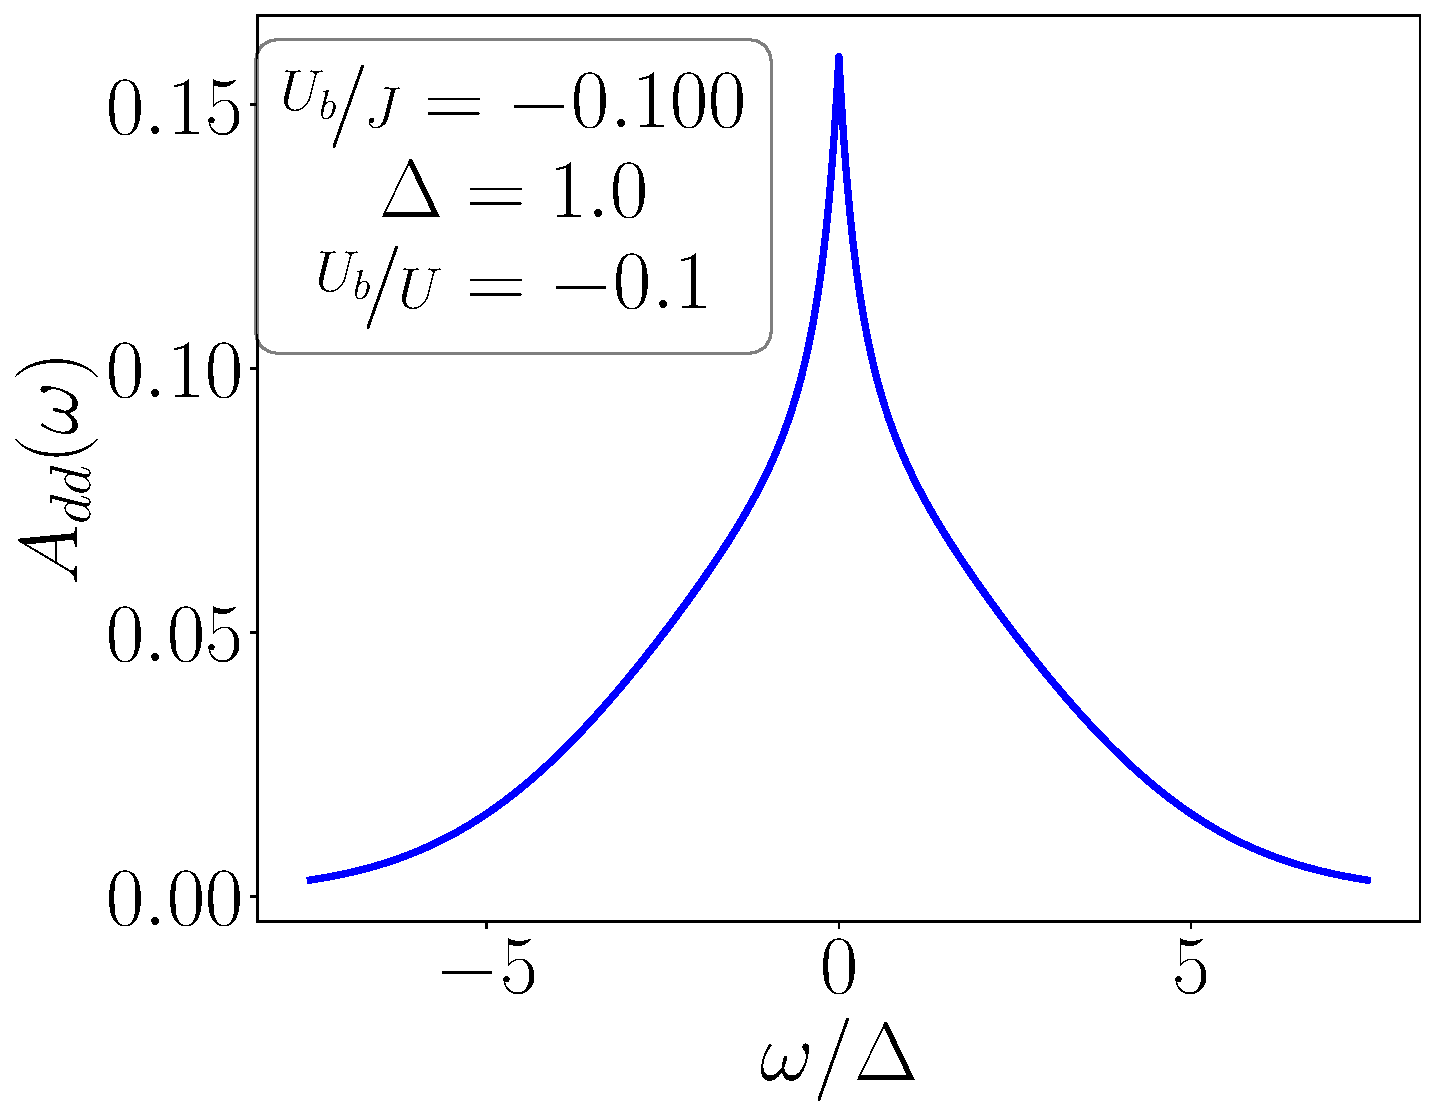
\includegraphics[width=0.2\textwidth]{../figures/spec_func_Ub_by_J=-0.100.pdf}
	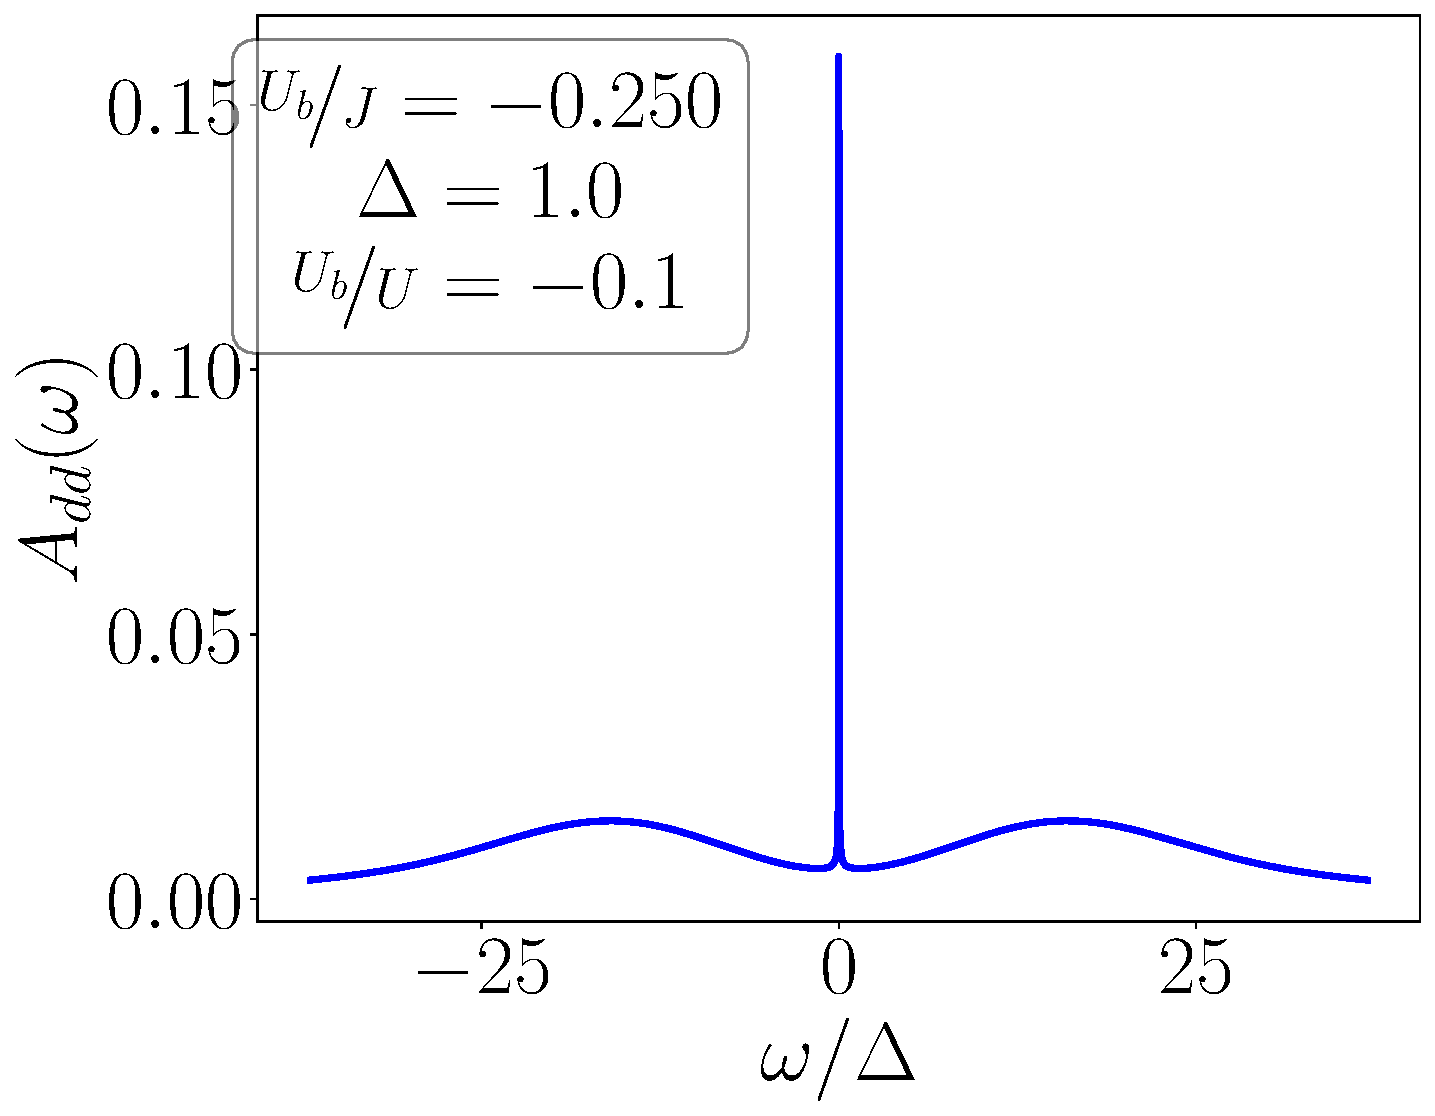
\includegraphics[width=0.2\textwidth]{../figures/spec_func_Ub_by_J=-0.250.pdf}
	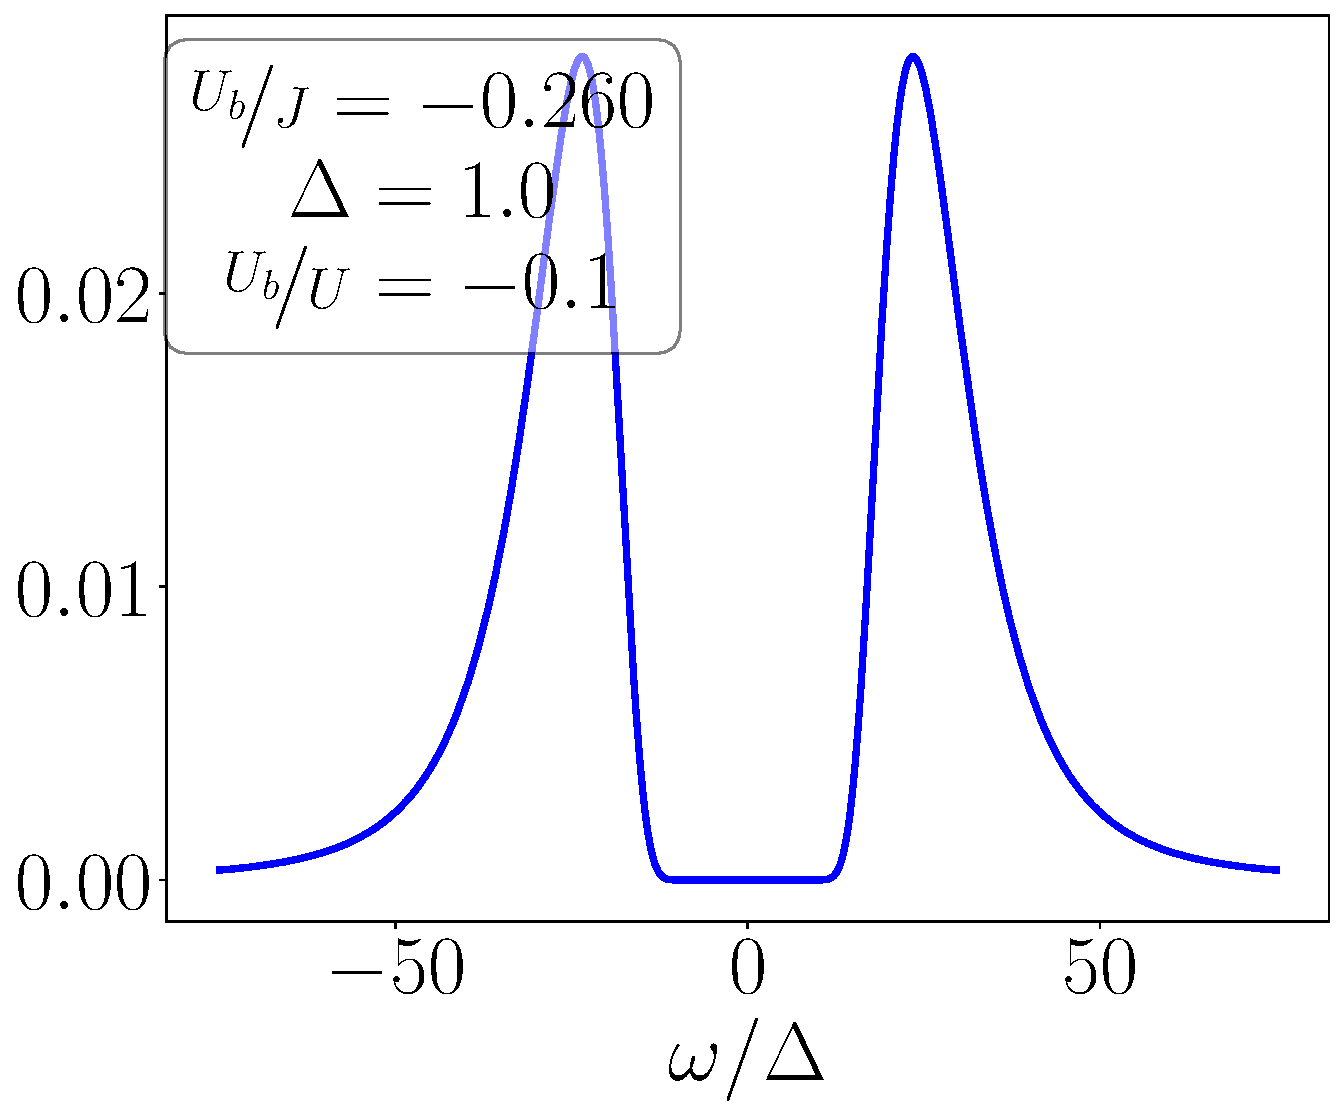
\includegraphics[width=0.2\textwidth]{../figures/spec_func_Ub_by_J=-0.26.pdf}
\end{center}

\section{Conclusions}

\begin{itemize}
	\item discuss why the model is minimal
\end{itemize}

\acknowledgments
Abhirup Mukherjee thanks IISER Kolkata for funding through a research fellowship. S. Lal thanks the SERB, Govt. of India for funding through MATRICS grant MTR/2021/000141 and Core Research Grant CRG/2021/000852.

\appendix*

\begin{widetext}
\section{Derivation of RG equations for the generalised Anderson impurity model}

\subsection{Renormalisation of the impurity energy \(\epsilon_d\)}
The coupling \(\epsilon_d\) is renormalised by three kinds of vertices: \(V^2\), \(J^2\) and \(K^2\). We will consider these processes one after another. We define \(n_j\) as the number of states being decoupled on each side of the Fermi surface, at the \(j^\text{th}\) RG step. In order to treat both spin and isospin exchanges democratically, we take \(\ket{\Psi}_i = \frac{1}{2}\left(\ket{0} + \ket{q\uparrow} + \ket{q\downarrow} + \ket{q\uparrow, q\downarrow}\right) \) as the \textit{initial} state for the scattering processes. The intermediate states \(\ket{\Psi}_\text{int}\) in the particle sector \(\left(c_{q\beta}\ket{\Psi}_i\right)\) and hole sector \(\left(c^\dagger_{q\beta}\ket{\Psi}_i\right)\) will then have both spin and isospin excitations which can couple with the corresponding impurity degree of freedom. We will assume that states  \(q > k_F~\left(\epsilon_q > 0\right) \) above the Fermi surface can have only particle excitations and states below the Fermi surface can only have hole excitations. The kinetic energy part \(\epsilon_q \tau_{q\beta}\) of \(H_D\) for \(\ket{\Psi}_i\) is then zero, whereas it is always \(D/2\) for \(\ket{\Psi}_\text{int}\). To demonstrate this for a typical \(q < k_F\), the hole excitation is \(c_{q \uparrow}\ket{\Psi}_i = \frac{1}{\sqrt 2}\left(\ket{0} + \ket{q \downarrow}\right)\). This has an isospin term in the form of the \textit{holon} and a spin term in the form of the down state. Since \(\tau_{q \uparrow} = -\frac{1}{2}\) in the excited state, the kinetic energy for \(\ket{\Psi}_\text{int}\) is \(\epsilon_q \tau_{q \uparrow} = \left(-D\right)\times\left(-\frac{1}{2}\right) = D/2\).

The renormalisation arising from the first kind of terms, in the particle sector, is
\begin{equation}\begin{aligned}
	\sum_{q\beta}c^\dagger_{q\beta}c_{d\beta}\frac{V^2}{\omega - H_D}c^\dagger_{d\beta}c_{q\beta} = \sum_{q\beta}V^2 \hat n_{q\beta} \left( 1 - \hat n_{d\beta} \right)\left( \frac{1-\hat n_{d \overline\beta }}{\omega - E_0} + \frac{\hat n_{d \overline\beta}}{\omega^\prime - E_1}\right) = V^2 n_j\sum_{\beta}\left( 1 - \hat n_{d\beta} \right)\left( \frac{1-\hat n_{d \overline\beta }}{\omega_0 - E_0} + \frac{\hat n_{d \overline\beta}}{\omega_1 - E_1}\right)
\end{aligned}\end{equation}
\(q\) runs over the momentum states that are being decoupled at this RG step: \(|q| = \Lambda_j\). \(E_{1,0}\) are the diagonal parts of the Hamiltonian at \(\hat n_{d\overline \beta}=1,0\) respectively. We have \(\hat n_{d\beta}=1\) in the intermediate state because of the \(c^\dagger_{d\beta}\) in front of the Greens function. Applying \(c_{q\beta}\) on the initial state \(\ket{\Psi}_i\) leaves us with \(C^z_q = - \frac{1}{2}\) and \(s^z_q = \frac{1}{2}\overline\beta\). We also know that
\begin{equation}\begin{aligned}
	\hat n_{d\beta}=1,
	\begin{cases}
		\hat n_{d\overline\beta}=0 &\implies S_d^z = \frac{1}{2}\beta, C_d^z = 0, \epsilon_d\left(\hat n_{d\uparrow} - \hat n_{d \downarrow}\right)^2 = \epsilon_d\\	
		\hat n_{d\overline\beta}=1 &\implies S_d^z = 0, C_d^z = \frac{1}{2}, \epsilon_d\left(\hat n_{d\uparrow} - \hat n_{d \downarrow}\right)^2 = 0
	\end{cases}
\end{aligned}\end{equation}
Combining all this, we can write \(E_1 = \frac{D}{2} - \frac{K}{4}\) and \(E_0 = \frac{D}{2} + \epsilon_d - \frac{J}{4}\). In order to relate \(\omega_0\) with \(\omega_1\) with the common fluctuation scale \(\omega\) for the conduction electrons, we will replace these quantum fluctuation scales by the current renormalised values of the single-particle self-energy for the initial state from which we started scattering. For \(\hat n_{d\overline\beta}=0\), there is no additional self-energy because the impurity does not have any spin: \(\omega_0 = \omega\). For \(\hat n_{d\overline\beta} = 1\), we have an additional self-energy of \(\epsilon_d\) arising from the correlation on the impurity: \(\omega_1 = \omega + \epsilon_d\).
Substituting the values of \(E_{0,1}\) and \(\omega_{0,1}\), we get
\begin{equation}\begin{aligned}
	\label{ren_ed_Vp}
	V^2 n_j\sum_{\beta}\left( 1 - \hat n_{d\beta} \right)\left( \frac{1-\hat n_{d \overline\beta }}{\omega - \frac{D}{2} - \epsilon_d + \frac{J}{4}} + \frac{\hat n_{d \overline\beta}}{\omega - \frac{D}{2} + \epsilon_d + \frac{K}{4}}\right)
\end{aligned}\end{equation}
Performing a similar calculation for the hole sector gives the contribution:
\begin{equation}\begin{aligned}
	\label{ren_ed_Vh}
	V^2 n_j\sum_{\beta}\hat n_{d\beta}\left( \frac{1-\hat n_{d \overline\beta }}{\omega - \frac{D}{2} + \epsilon_d + \frac{K}{4}} + \frac{\hat n_{d \overline\beta}}{\omega - \frac{D}{2} - \epsilon_d + \frac{J}{4}}\right)
\end{aligned}\end{equation}
We now come to the second type of terms: spin-spin. We first look at the particle sector:
\begin{equation}\begin{aligned}
	\label{ren_ed_Jpp}
	\frac{J^2}{4}\sum_{q\beta}c^\dagger_{d\overline\beta}c_{d\beta}c^\dagger_{q\beta}c_{-q\overline\beta} \frac{1}{\omega - H_D}c^\dagger_{d\beta}c_{d\overline\beta}c^\dagger_{q\overline\beta}c_{q\beta} = \frac{J^2}{4} n_j\frac{1}{\omega - \frac{D}{2} + \frac{J}{4}} \sum_{\beta}\hat n_{d\overline\beta}\left( 1 - \hat n_{d\beta} \right)
\end{aligned}\end{equation}
The diagonal part in the denominator was simple to deduce in this case, because the nature of the scattering requires the spins \(S_d^z\) and \(\frac{\beta}{2}\left(\hat n_{q\beta} - \hat n_{q \overline\beta}\right)\) to be anti-parallel. This ensures that the intermediate state has an energy of \(E = \frac{D}{2} + \epsilon_d - \frac{J}{4}\), and the quantum fluctuation scale is \(\omega^\prime = \omega + \epsilon_d\), such that \(\omega^\prime - E = \omega - \frac{D}{2} + \frac{J}{4}\). In the hole sector, we have
\begin{equation}\begin{aligned}
	\label{ren_ed_Jph}
	\frac{J^2}{4} n_j\frac{1}{\omega - \frac{D}{2} + \frac{J}{4}} \sum_{\beta}\hat n_{d\beta}\left( 1 - \hat n_{d\overline\beta} \right)
\end{aligned}\end{equation}
The final kind of scattering is the \(K^2\) type. Similar to the \(J^2\) term, we get the following contribution:
\begin{equation}\begin{aligned}
	\label{ren_ed_Kpp}
	\frac{K^2}{4}\sum_{q\beta}c^\dagger_{q\beta}c^\dagger_{q\overline\beta}c_{d\overline\beta}c_{d\beta} \frac{1}{\omega - H_D}c^\dagger_{d\beta}c^\dagger_{d\overline\beta}c_{q\overline\beta}c_{q\beta} = \frac{K^2}{2} n_j\frac{1}{\omega - \frac{D}{2} + \frac{K}{4}} \left(1 - \hat n_{d \uparrow}\right) \left( 1 - \hat n_{d \downarrow} \right)
\end{aligned}\end{equation}
in the particle sector. This is again because \(E = \frac{D}{2} - \frac{K}{4}\) in the intermediate state and \(\omega^\prime = \omega\). In the hole sector, we get
\begin{equation}\begin{aligned}
	\label{ren_ed_Kph}
	\frac{K^2}{2} n_j\frac{1}{\omega - \frac{D}{2} + \frac{K}{4}} \hat n_{d\uparrow}\hat n_{d \downarrow}~.
\end{aligned}\end{equation}

We now have all possible renormalisation to the impurity energy \(\epsilon_d\). To actually compute the renormalisation, we will first calculate the renormalisation in the energies \(\epsilon_0, \epsilon_1\) and \(\epsilon_2\) of the impurity states \(\ket{\hat n_d = 0}, \ket{\hat n_d = 1}, \ket{\hat n_d = 2}\) respectively. The renormalisation of these states are given by the following terms:
\begin{itemize}
	\item \(\Delta \epsilon_0\) is given by the renormalisation of the term \(\left(1 - \hat n_{d\uparrow}\right)\left(1 - \hat n_{d \downarrow}\right)\)
	\item \(\Delta \epsilon_1\) is given by the renormalisation of either \(\left(1 - \hat n_{d\uparrow}\right)\hat n_{d \downarrow}\) or \(\left(1 - \hat n_{d\downarrow}\right)\hat n_{d \uparrow}\)
	\item \(\Delta \epsilon_2\) is given by the renormalisation of \(\hat n_{d\uparrow}\hat n_{d \downarrow}\)
\end{itemize}
From eqs.~\ref{ren_ed_Vp}, \ref{ren_ed_Vh}, \ref{ren_ed_Jpp}, \ref{ren_ed_Jph}, \ref{ren_ed_Kpp} and \ref{ren_ed_Kph}, we write
\begin{equation}\begin{aligned}
	\Delta \epsilon_0 = \Delta \epsilon_2 = \frac{2V^2 n_j}{\omega - \frac{D}{2} - \epsilon_d + \frac{J}{4}} + \frac{K^2 n_j/2}{\omega - \frac{D}{2} + \frac{K}{4}}, && \Delta \epsilon_1 = \frac{2V^2 n_j}{\omega - \frac{D}{2} + \epsilon_d + \frac{K}{4}} + \frac{J^2 n_j/2}{\omega - \frac{D}{2} + \frac{J}{4}}
\end{aligned}\end{equation}
We had started with a particle-hole symmetric Hamiltonian \((2\epsilon_d + U = 0)\); the fact that \(\Delta \epsilon_0 = \Delta \epsilon_2\) means the RG transformation has preserved that symmetry. The renormalisation of \(\epsilon_d\) is simply the renormalisation in the energy difference between the singly-occupied and vacant impurity levels: \(\Delta \epsilon_d = \Delta \epsilon_1 - \Delta \epsilon_0\). This gives our first RG equation:
\begin{equation}\begin{aligned}
	\Delta \epsilon_d = 2V^2 n_j\left(\frac{1}{\omega - \frac{D}{2} + \epsilon_d + \frac{K}{4}} - \frac{1}{\omega - \frac{D}{2} - \epsilon_d + \frac{J}{4}}\right) + \frac{n_j}{2}\left(\frac{J^2}{\omega - \frac{D}{2} + \frac{J}{4}} - \frac{K^2}{\omega - \frac{D}{2} + \frac{K}{4}}\right)
\end{aligned}\end{equation}

\subsection{Renormalisation of the hybridisation \(V\)}
Renormalisation of \(V\) happens through two kinds of processes: \(VJ\) and \(VK\). In order words, the two vertices involve one single-particle scattering and one spin or isospin exchange respectively. We first look at the vertices that involve a spin-exchange scattering.

Within spin-exchange, the scattering can be either via \(S_d^z\) or through \(S_d^\pm\). For the first kind, we have the following contribution in the particle sector:
\begin{equation}\begin{aligned}
	\sum_{q\beta} Vc^\dagger_{q\beta} c_{d\beta} \frac{1}{\omega - H_D}\frac{1}{4}J \sum_{k} \left(\hat n_{d\beta} - \hat n_{d\overline\beta}\right) c^\dagger_{k\beta}c_{q\beta} = \frac{1}{4}V J n_j \frac{1}{2}\left(\frac{1}{\omega^\prime_1 - E} + \frac{1}{\omega^\prime_2 - E}\right)\sum_{k\beta} \left(1 - \hat n_{d\overline\beta}\right) c_{d\beta}c^\dagger_{k\beta}
\end{aligned}\end{equation}
The transformation from \(\frac{1}{\omega - H_D}\) to \(\frac{1}{2}\left(\frac{1}{\omega^\prime_1 - E} + \frac{1}{\omega^\prime_2 - E}\right)\) is made so that we can account for both the initial state and the final state energies through the two fluctuation scales \(\omega^\prime_1\) and \(\omega_2^\prime\) respectively; we calculate the denominators for both the initial and final states, and then take the mean of the two (hence the factor of half in front). This was not required previously because in the earlier scattering processes, the impurity returned to its initial state at the end, at least in terms of \(\epsilon_d \left( \hat n_{d \uparrow} - \hat n_{d \downarrow} \right)^2 \), and so we had \(\omega_1^\prime = \omega_2^\prime = \omega^\prime\).

Note that the \(c_{d\beta}\) in front of the Greens function resulted in \(\left(\hat n_{d\beta} - \hat n_{d\overline\beta}\right) \to \left(1 - \hat n_{d\overline\beta}\right)\). The intermediate state is characterised by \(\hat n_{d\beta} = 1 - \hat n_{d \overline \beta} = 1\), which means that \(E = \frac{D}{2} + \epsilon_d - \frac{J}{4}\). Moreover, the initial state gives \(\omega_1^\prime = \omega + \epsilon_d\) while the final state gives \(\omega^\prime_2 = \omega\). Therefore, the renormalisation becomes
\begin{equation}\begin{aligned}
	-\frac{n_j}{4}V J \frac{1}{2}\left(\frac{1}{\omega - \frac{D}{2} + \frac{J}{4}} + \frac{1}{\omega - \frac{D}{2} - \epsilon_d + \frac{J}{4}}\right)\sum_{k\beta}\left(1 - \hat n_{d\overline\beta}\right) c^\dagger_{k\beta} c_{d\beta}
\end{aligned}\end{equation}
One can generate another such process by exchanging the single-particle process and the spin-exchange process:
\begin{equation}\begin{aligned}
	\sum_{q\beta} \frac{1}{4}J \sum_{k} \left(\hat n_{d\beta} - \hat n_{d\overline\beta}\right) c^\dagger_{q\beta}c_{k\beta} \frac{1}{\omega - H_D} V c^\dagger_{d\beta} c_{q\beta}
\end{aligned}\end{equation}
This is simply the Hermitian conjugate of the previous contribution. Combining this with the previous then gives
\begin{equation}\begin{aligned}
	-\frac{n_j}{8}V J \left(\frac{1}{\omega - \frac{D}{2} + \frac{J}{4}} + \frac{1}{\omega - \frac{D}{2} - \epsilon_d + \frac{J}{4}}\right) \sum_{k\beta}\left(1 - \hat n_{d\overline\beta}\right)\left(c^\dagger_{d\beta} c_{k\beta} + \text{h.c.}\right)
\end{aligned}\end{equation}

We now consider the spin-exchange processes involving \(S_d^\pm\):
\begin{equation}\begin{aligned}
	\sum_{q\beta} Vc^\dagger_{q\beta} c_{d\beta} \frac{1}{\omega - H_D}\frac{1}{2}J \sum_{k} c^\dagger_{d\beta}c_{d\overline\beta} c^\dagger_{k\overline\beta}c_{q\beta} = \frac{1}{2}V J n_j \frac{1}{2}\left(\frac{1}{\omega^\prime_1 - E} + \frac{1}{\omega^\prime_2 - E}\right) \sum_{k\beta} \left(1 - \hat n_{d\beta}\right) c_{d\overline\beta}c^\dagger_{k\overline\beta}
\end{aligned}\end{equation}
We again have \(E = \frac{D}{2} + \epsilon_d - \frac{J}{4},\omega_1^\prime = \omega + \epsilon_d\) and \(\omega_2^\prime = \omega\), which gives
\begin{equation}\begin{aligned}
	-\frac{1}{4}V J n_j \left(\frac{1}{\omega - \frac{D}{2} + \frac{J}{4}} + \frac{1}{\omega - \frac{D}{2} - \epsilon_d + \frac{J}{4}}\right) \sum_{k\beta} \left(1 - \hat n_{d\beta}\right)c^\dagger_{k\overline\beta} c_{d\overline\beta}
\end{aligned}\end{equation}
Combining this with the Hermitian conjugate obtained from exchanging the processes gives
\begin{equation}\begin{aligned}
	-\frac{1}{4}V J n_j \left(\frac{1}{\omega - \frac{D}{2} + \frac{J}{4}} + \frac{1}{\omega - \frac{D}{2} - \epsilon_d + \frac{J}{4}}\right) \sum_{k\beta} \left(1 - \hat n_{d\beta}\right)\left(c^\dagger_{k\overline\beta} c_{d\overline\beta} + \text{h.c.}\right)
\end{aligned}\end{equation}

The contributions from the hole sector are obtained making the transformation \(\hat n_{d\overline\beta} \to 1 - \hat n_{d\overline\beta}\) on the particle sector contributions. The total renormalisation to \(V\) from \(VJ\) processes are
\begin{equation}\begin{aligned}
	-\frac{3n_j}{8}V J \left(\frac{1}{\omega - \frac{D}{2} + \frac{J}{4}} + \frac{1}{\omega - \frac{D}{2} - \epsilon_d + \frac{J}{4}}\right) \sum_{k\beta}\left(c^\dagger_{d\beta} c_{k\beta} + \text{h.c.}\right)
\end{aligned}\end{equation}

We now look at the \(VK\) processes. The first one is
\begin{equation}\begin{aligned}
	\sum_{q\beta} Vc^\dagger_{q\beta} c_{d\beta} \frac{1}{\omega - H_D}\frac{1}{4}K \sum_{k} \left(\hat n_{d} - 1\right) c^\dagger_{k\beta}c_{q\beta} = -\frac{1}{8}V K n_j \left(\frac{1}{\omega - \frac{D}{2} + \frac{K}{4}} + \frac{1}{\omega - \frac{D}{2} + \epsilon_d + \frac{K}{4}}\right) \sum_{k\beta} \hat n_{d\overline \beta}c^\dagger_{k\beta}c_{d\beta}
\end{aligned}\end{equation}
The exchanged process again gives the Hermitian conjugate, so the combined contribution is
\begin{equation}\begin{aligned}
	-\frac{1}{8}V K n_j \left(\frac{1}{\omega - \frac{D}{2} + \frac{K}{4}} + \frac{1}{\omega - \frac{D}{2} + \epsilon_d + \frac{K}{4}}\right) \sum_{k\beta} \hat n_{d\overline \beta} \left(c^\dagger_{k\beta}c_{d\beta} + \text{h.c.}\right)
\end{aligned}\end{equation}

The isospin-flip vertex gives
\begin{equation}\begin{aligned}
	\sum_{q\beta} V c^\dagger_{q\beta} c_{d\beta} \frac{1}{\omega - H_D}\frac{1}{2}K \sum_{k} c^\dagger_{d\beta}c^\dagger_{d\overline\beta} c_{k\overline\beta} c_{q\beta} = \frac{1}{4}K V n_j \left(\frac{1}{\omega - \frac{D}{2} + \frac{K}{4}} + \frac{1}{\omega - \frac{D}{2} + \epsilon_d + \frac{K}{4}}\right) \sum_{k\beta} \left(1 - \hat n_{d\beta}\right) c^\dagger_{d\overline\beta}c_{k\overline\beta}~.
\end{aligned}\end{equation}
Combining with Hermitian conjugate gives
\begin{equation}\begin{aligned}
	\frac{1}{4}K V n_j \left(\frac{1}{\omega - \frac{D}{2} + \frac{K}{4}} + \frac{1}{\omega - \frac{D}{2} + \epsilon_d + \frac{K}{4}}\right) \sum_{k\beta} \left(1 - \hat n_{d\beta}\right) \left(c^\dagger_{d\overline\beta}c_{k\overline\beta} + \text{h.c.}\right)~.
\end{aligned}\end{equation}

After obtaining the hole sector contributions, the total renormalisation from \(VK\) processes is
\begin{equation}\begin{aligned}
	-\frac{3n_j}{4}V K \left(\frac{1}{\omega - \frac{D}{2} + \frac{K}{4}} + \frac{1}{\omega - \frac{D}{2} + \epsilon_d + \frac{K}{4}}\right) \sum_{k\beta}\left(c^\dagger_{d\beta} c_{k\beta} + \text{h.c.}\right)~.
\end{aligned}\end{equation}

The RG equation for \(V\) is
\begin{equation}\begin{aligned}
	\Delta V = -\frac{3n_j V}{8}\left[J\left(\frac{1}{\omega - \frac{D}{2} + \frac{J}{4}} + \frac{1}{\omega - \frac{D}{2} - \epsilon_d + \frac{J}{4}}\right) + K \left(\frac{1}{\omega - \frac{D}{2} + \frac{K}{4}} + \frac{1}{\omega - \frac{D}{2} + \epsilon_d + \frac{K}{4}}\right)\right]
\end{aligned}\end{equation}

\subsection{Renormalisation of the exchange couplings \(J\) and \(K\)}
We will just note the renormalisation in \(J^z\), which will be equal to \(J^\pm\) due to spin-rotation symmetry. The terms that renormalise \(J^z\) are of the form \(S_d^\pm S_d^\mp\). In the particle sector, we have
\begin{equation}\begin{aligned}
	\sum_{q} \sum_{kk^\prime}\frac{1}{4}J^2 S_d^\pm c^\dagger_{q\mp}c_{k^\prime\pm} \frac{1}{\omega - H_D}S_d^\mp c^\dagger_{k\pm}c_{q\mp} = -n_j \frac{1}{4}J^2 \left(\frac{1}{2} \pm S_d^z\right) \sum_{kk^\prime}c^\dagger_{k \pm}c_{k\pm} \frac{1}{\omega - \frac{D}{2} + \frac{J}{4}}~.
\end{aligned}\end{equation}
The denominator is determined using \(E = \frac{D}{2} + \epsilon_d - \frac{J}{4}\) and \(\omega^\prime = \omega + \epsilon_d\).
In the hole sector, we similarly have
\begin{equation}\begin{aligned}
	\sum_{q} \sum_{kk^\prime}\frac{1}{4}J^2 S_d^\mp c^\dagger_{k\pm}c_{q\mp} \frac{1}{\omega - H_D}S_d^\pm c^\dagger_{q\mp}c_{k^\prime\pm} = n_j \frac{1}{4}J^2 \left(\frac{1}{2} \mp S_d^z\right) \sum_{kk^\prime}c^\dagger_{k \pm}c_{k\pm} \frac{1}{\omega - \frac{D}{2} + \frac{J}{4}}~.
\end{aligned}\end{equation}
Adding all four expressions and dropping the constant part, we get
\begin{equation}\begin{aligned}
	-n_j \frac{1}{2}J^2 S_d^z \sum_{kk^\prime}\left(c^\dagger_{k \uparrow}c_{k^\prime \uparrow} - c^\dagger_{k \downarrow}c_{k^\prime \downarrow}\right) \frac{1}{\omega - \frac{D}{2} + \frac{J}{4}}~.
\end{aligned}\end{equation}
We can now directly read off the RG equation for \(J\):
\begin{equation}\begin{aligned}
	\Delta J = -\frac{n_j J^2}{\omega - \frac{D}{2} + \frac{J}{4}}
\end{aligned}\end{equation}

Since the spin and charge degrees of freedom are treated on an equal footing in the model, we obtain the RG equation for \(K\) by simply changing \(J \to K\):
\begin{equation}\begin{aligned}
	\Delta K = -\frac{n_j K^2}{\omega - \frac{D}{2} + \frac{K}{4}}
\end{aligned}\end{equation}

\section{\(U_b\)-included terms}

We first Fourier transform the \(U_b\)-term to \(k-\)space. In \(k-\)space, the diagonal contribution (to \(H_D\)) coming from this term is the single-particle self-energy \(-U_b\left(\hat n_{q \beta}\right)^2\) which can be made particle-hole symmetric in the form:
\begin{equation}\begin{aligned}
	-U_b\left(\tau_{q \beta}\right)^2
\end{aligned}\end{equation}
where \(q\) is the \(k-\)state being decoupled and \(\tau \equiv \hat n - 1/2\). In the initial state \(\ket{\Psi}_i\), we have \(\langle \hat n_{q\beta} \rangle = 1/2 \implies \tau_{q\beta} = 0\), so the contribution of \(U_b\) to that state is 0. For both hole excitations \(c_{q\beta}\ket{\Psi}_i\) as well as particle excitations \(c^\dagger_{q\beta}\ket{\Psi}_i\), the intermediate state energy lowers to \(-U_b/4\).

The off-diagonal part is
\begin{equation}\begin{aligned}
	-\frac{U_b}{2}\sum_{kk^\prime\sigma}c^\dagger_{k\sigma}c_{k^\prime\sigma} + U_b \sum_{k_1,k_2,k_1^\prime,k_2^\prime} c^\dagger_{k_1 \uparrow}c_{k_2 \uparrow} c^\dagger_{k^\prime_1 \downarrow}c_{k^\prime_2 \downarrow} 
\end{aligned}\end{equation}
We ignore the potential scattering arising from the first term.

\subsection{Renormalisation of \(U_b\)}
\(U_b\) can renormalise only via itself. The relevant renormalisation term in the particle sector is
\begin{equation}\begin{aligned}
	U_b^2 \sum_{q\beta}\sum_{k_1,k_2,k_3,k_1^\prime,k_2^\prime,k_3^\prime} c^\dagger_{q\beta}c_{k_1\beta}c^\dagger_{k_3\overline\beta}c_{k_1^\prime\overline\beta}\frac{1}{\omega - H_D}c^\dagger_{k_2^\prime\overline\beta}c_{k_3^\prime\overline\beta}c^\dagger_{k_2\beta}c_{q\beta}
\end{aligned}\end{equation}
In order to renormalise \(U_b\), we need to contract one more pair of momenta. There are two choices. The first is by setting \(k_3 = k_3^\prime = q\). The two internal states, then, are \(q\beta\) and \(q\overline\beta\). As discussed above, the intermediate state energy is \(-U_b/4\). We therefore have
\begin{equation}\begin{aligned}
	\frac{U_b^2 n_j}{\omega - D/2 + U_b/4}\sum_{\beta}\sum_{k_1,k_2,k_1^\prime,k_2^\prime} c_{k_1\beta}c_{k_1^\prime\overline\beta}c^\dagger_{k_2^\prime\overline\beta}c^\dagger_{k_2\beta} = \frac{U_b^2 n_j}{\omega - D/2 + U_b/4}\sum_{\beta}\sum_{k_1,k_2,k_1^\prime,k_2^\prime} c^\dagger_{k_2^\prime\overline\beta}c_{k_1^\prime\overline\beta}c^\dagger_{k_2\beta}c_{k_1\beta}
\end{aligned}\end{equation}
Another way to contract the momenta is by setting \(k_1^\prime = k_2^\prime = q\), which gives a renormalisation of
\begin{equation}\begin{aligned}
	\frac{U_b^2 n_j}{\omega - D/2 + U_b/4}\sum_{\beta}\sum_{k_1,k_2,k_3,k_3^\prime} c_{k_1\beta}c^\dagger_{k_3 \overline\beta}c_{k_3\prime\overline\beta}c^\dagger_{k_2\beta} = -\frac{U_b^2 n_j}{\omega - D/2}\sum_{\beta}\sum_{k_1,k_2,k_3,k_3^\prime} c^\dagger_{k_3 \overline\beta}c_{k_3\prime\overline\beta}c^\dagger_{k_2\beta}c_{k_1\beta}
\end{aligned}\end{equation}
The two contributions cancel each other. The same cancellation happens in the hole sector as well.

\subsection{Renormalisation of \(U\)}
\(U_b\) does not have any new renormalisation term on account of \(U_b\). \(U_b\) does however modify the existing RG equation for \(U\), by shifting the denominator. The existing RG equation is
\begin{equation}\begin{aligned}
	\Delta U &= -4V^2 n_j\left(\frac{1}{\omega - \frac{D}{2} + \epsilon_d + \frac{K}{4}} - \frac{1}{\omega - \frac{D}{2} - \epsilon_d + \frac{J}{4}}\right) - n_j\left(\frac{J^2}{\omega - \frac{D}{2} + \frac{J}{4}} - \frac{K^2}{\omega - \frac{D}{2} + \frac{K}{4}}\right)~.
\end{aligned}\end{equation}
On accounting for the contribution of \(U_b\) to the denominator, we get
\begin{equation}\begin{aligned}
	\Delta U &= -4V^2 n_j\left(\frac{1}{\omega - \frac{D}{2} + \frac{U_b}{4} + \epsilon_d + \frac{K}{4}} - \frac{1}{\omega - \frac{D}{2} + \frac{U_b}{4} - \epsilon_d + \frac{J}{4}}\right) - n_j\left(\frac{J^2}{\omega - \frac{D}{2} + \frac{U_b}{4} + \frac{J}{4}} - \frac{K^2}{\omega - \frac{D}{2} + \frac{U_b}{4} + \frac{K}{4}}\right)~.
\end{aligned}\end{equation}

\subsection{Renormalisation of \(V\)}
The single-particle  hybridisation \(V\) renormalises through terms of \(V U_b\) and \(U_b V\) kind. The first term gives
\begin{equation}\begin{aligned}
	&\sum_{q\beta}\sum_{k}U_b V c^\dagger_{q\beta}c_{k\beta} \hat n_{q\overline\beta} \frac{1}{\omega - H_D} c^\dagger_{d\beta}c_{q\beta} \\
	&= n_jU_b V\sum_{k\beta} c_{k\beta} \left[\frac{\hat n_{d\overline\beta}}{2}\left(\frac{1}{\omega_1 - E_1} + \frac{1}{\omega^\prime_1 - E_1}\right) + \frac{1-\hat n_{d\overline\beta}}{2}\left(\frac{1}{\omega_0 - E_0} + \frac{1}{\omega_0^\prime - E_0}\right)\right] c^\dagger_{d\beta}
\end{aligned}\end{equation}
\(E_1\) and \(E_0\) are the intermediate state energies for \(\hat n_{d\overline\beta}=1\) and 0 respectively. \(\omega_{1,0}\) are the quantum fluctuation scales for the corresponding initial states. \(\omega^\prime_{1,0}\) are the fluctuation scales for the corresponding final states.
The intermediate energies are \(E_1 = D/2 - U_b/4 - K/4,~ ~ ~ E_0 = D/2 - U_b/4 - U/2 - J/4\). The fluctuation scales are \(\omega_1 = \omega - U/2= \omega_0^\prime,~ ~ ~ \omega_1^\prime = \omega = \omega_0\). Substituting these gives
\begin{equation}\begin{aligned}
	-n_jU_b V\sum_{k\beta} c^\dagger_{d\beta} c_{k\beta} \left[\frac{\hat n_{d\overline\beta}}{2}\left(\frac{1}{\omega - \frac{D}{2} - \frac{U}{2} + \frac{U_b}{4} + \frac{K}{4}} + \frac{1}{\omega - \frac{D}{2} + \frac{U_b}{4} + \frac{K}{4}}\right) \right.\\
+\left. \frac{1-\hat n_{d\overline\beta}}{2}\left(\frac{1}{\omega - \frac{D}{2} + \frac{U_b}{4} + \frac{U}{2} + \frac{J}{4}} + \frac{1}{\omega - \frac{D}{2} + \frac{U_b}{4} + \frac{J}{4}}\right)\right]
\end{aligned}\end{equation}

The second term is of the form
\begin{equation}\begin{aligned}
	\sum_{q\beta}\sum_{k}U_b V c^\dagger_{q\beta}c_{d\beta} \frac{1}{\omega - H_D} \hat n_{q\overline\beta} c^\dagger_{k\beta}c_{q\beta}
\end{aligned}\end{equation}
and this is just the Hermitian conjugate of the previous term, so these two terms together lead to
\begin{equation}\begin{aligned}
	-n_jU_b V\sum_{k\beta} \left(c^\dagger_{d\beta} c_{k\beta} + \text{h.c.}\right) \left[\frac{\hat n_{d\overline\beta}}{2}\left(\frac{1}{\omega - \frac{D}{2} - \frac{U}{2} + \frac{U_b}{4} + \frac{K}{4}} + \frac{1}{\omega - \frac{D}{2} + \frac{U_b}{4} + \frac{K}{4}}\right) \right.\\
	+ \left.\frac{1-\hat n_{d\overline\beta}}{2}\left(\frac{1}{\omega - \frac{D}{2} + \frac{U_b}{4} + \frac{U}{2} + \frac{J}{4}} + \frac{1}{\omega - \frac{D}{2} + \frac{U_b}{4} + \frac{J}{4}}\right)\right]
\end{aligned}\end{equation}

In the hole sector, we have
\begin{equation}\begin{aligned}
	&\sum_{q\beta}\sum_{k}U_b V \hat n_{q\overline\beta} c^\dagger_{k\beta}c_{q\beta} \frac{1}{\omega - H_D} c^\dagger_{q\beta}c_{d\beta}\\
	&-\sum_{q\beta}\sum_{k}U_b V \left(1 - \hat n_{q\overline\beta}\right) c^\dagger_{k\beta}c_{q\beta} \frac{1}{\omega - H_D} c^\dagger_{q\beta}c_{d\beta}\\
	&= -n_jU_b V\sum_{k\beta} c^\dagger_{k\beta} \left[\frac{\hat n_{d\overline\beta}}{2}\left(\frac{1}{\omega_1 - E_1} + \frac{1}{\omega^\prime_1 - E_1}\right) + \frac{1-\hat n_{d\overline\beta}}{2}\left(\frac{1}{\omega_0 - E_0} + \frac{1}{\omega_0^\prime - E_0}\right)\right] c_{d\beta}
\end{aligned}\end{equation}
\(E_1 = D/2 - U_b/4 - U/2 - J/4,~ ~ ~ E_0 = D/2 - U_b/4 - K/4\). The fluctuation scales are \(\omega_1 = \omega = \omega_0^\prime,~ ~ ~ \omega_1^\prime = \omega - U/2 = \omega_0\). Substituting these gives
\begin{equation}\begin{aligned}
	-n_jU_b V\sum_{k\beta} c^\dagger_{d\beta} c_{k\beta} \left[\frac{1 - \hat n_{d\overline\beta}}{2}\left(\frac{1}{\omega - \frac{D}{2} - \frac{U}{2} + \frac{U_b}{4} + \frac{K}{4}} + \frac{1}{\omega - \frac{D}{2} + \frac{U_b}{4} + \frac{K}{4}}\right) \right.\\
+\left. \frac{\hat n_{d\overline\beta}}{2}\left(\frac{1}{\omega - \frac{D}{2} + \frac{U_b}{4} + \frac{U}{2} + \frac{J}{4}} + \frac{1}{\omega - \frac{D}{2} + \frac{U_b}{4} + \frac{J}{4}}\right)\right]
\end{aligned}\end{equation}
The other term, obtained by exchanging \(V\) and \(U_b\), gives the Hermitian conjugate, so the overall contribution from the hole sector is the same as the total contribution from the particle sector, but with \(\hat n_{d\overline\beta} \to 1 - \hat n_{d\overline\beta}\). Combining both the sectors, we get
\begin{equation}\begin{aligned}
	-n_jU_b V\sum_{k\beta} \left(c^\dagger_{d\beta} c_{k\beta} + \text{h.c.}\right) \frac{1}{2}\left[\left(\frac{1}{\omega - \frac{D}{2} - \frac{U}{2} + \frac{U_b}{4} + \frac{K}{4}} + \frac{1}{\omega - \frac{D}{2} + \frac{U_b}{4} + \frac{K}{4}}\right) \right.\\
+\left. \left(\frac{1}{\omega - \frac{D}{2} + \frac{U_b}{4} + \frac{U}{2} + \frac{J}{4}} + \frac{1}{\omega - \frac{D}{2} + \frac{U_b}{4} + \frac{J}{4}}\right)\right]
\end{aligned}\end{equation}

Combining with the already existing RG equations, the complete RG equation for \(V\) becomes
\begin{equation}\begin{aligned}
	\Delta V =& -\frac{3n_j V}{8}\left[\left(\frac{J}{\omega - \frac{D}{2} + \frac{U_b}{4} + \frac{J}{4}} + \frac{J}{\omega - \frac{D}{2} + \frac{U_b}{4} + \frac{U}{2} + \frac{J}{4}}\right) + K \left(\frac{K}{\omega - \frac{D}{2} + \frac{U_b}{4} + \frac{K}{4}} + \frac{K}{\omega - \frac{D}{2} + \frac{U_b}{4} - \frac{U}{2} + \frac{K}{4}}\right)\right]\\
		 &-\frac{n_jU_b}{2}\left[\left(\frac{V}{\omega - \frac{D}{2} - \frac{U}{2} + \frac{U_b}{4} + \frac{K}{4}} + \frac{V}{\omega - \frac{D}{2} + \frac{U_b}{4} + \frac{K}{4}}\right) + \left(\frac{V}{\omega - \frac{D}{2} + \frac{U_b}{4} + \frac{U}{2} + \frac{J}{4}} + \frac{V}{\omega - \frac{D}{2} + \frac{U_b}{4} + \frac{J}{4}}\right)\right]\\
		 &=-\frac{n_j V}{8}\left[\left(\frac{3J + 4U_b}{\omega - \frac{D}{2} + \frac{U_b}{4} + \frac{J}{4}} + \frac{3J + 4U_b}{\omega - \frac{D}{2} + \frac{U_b}{4} + \frac{U}{2} + \frac{J}{4}}\right) + \left(\frac{3K + 4U_b}{\omega - \frac{D}{2} + \frac{U_b}{4} + \frac{K}{4}} + \frac{3K + 4U_b}{\omega - \frac{D}{2} + \frac{U_b}{4} - \frac{U}{2} + \frac{K}{4}}\right)\right]
\end{aligned}\end{equation}

\subsection{Renormalisation of \(J\) and \(K\)}
We will track the entire renormalisation purely from that of \(J^+\), by virtue of the SU(2) symmetry. \(J^+\) renormalises through the \(J U_b\) terms. One of the terms is
\begin{equation}\begin{aligned}
	\frac{1}{2} J U_b \sum_{q} \sum_{k,k^\prime} S_d^+ c^\dagger_{q \downarrow} c_{k \uparrow} \frac{1}{\omega - H_D} \hat n_{q \uparrow} c^\dagger_{k^\prime \downarrow}c_{q \downarrow} = -\frac{1}{2}\frac{J U_b n_j}{\omega - \frac{D}{2} + \frac{U_b}{2} + \frac{J}{4}} \sum_{k,k^\prime} S_d^+ c^\dagger_{k^\prime \downarrow} c_{k \uparrow}
\end{aligned}\end{equation}
The factor of half in front is the same half factor that appears in front of the \(S_1^+ S_2^-, S_1^-S_2^+\) terms when we rewrite \(\vec{S}_1\cdot\vec{S}_2\) in terms of \(S^z, S^\pm\). Another term is obtained by switching \(J\) and \(U_b\):
\begin{equation}\begin{aligned}
	\frac{1}{2} J U_b \sum_{q} \sum_{k,k^\prime} \hat n_{q \downarrow} c^\dagger_{q \uparrow} c_{k \uparrow} \frac{1}{\omega - H_D}S_d^+ c^\dagger_{k^\prime \downarrow} c_{q \uparrow} = -\frac{1}{2}\frac{J U_b n_j}{\omega - \frac{D}{2} + \frac{U_b}{2} + \frac{J}{4}} \sum_{k,k^\prime} S_d^+ c^\dagger_{k^\prime \downarrow} c_{k \uparrow}
\end{aligned}\end{equation}

The corresponding terms in the hole sector are
\begin{equation}\begin{aligned}
	\frac{1}{2} J U_b \sum_{q} \sum_{k,k^\prime} S_d^+ c^\dagger_{k^\prime \downarrow} c_{q \uparrow} \frac{1}{\omega - H_D} \hat n_{q \downarrow} c^\dagger_{q \uparrow}c_{k \uparrow} = -\frac{1}{2}\frac{J U_b n_j}{\omega - \frac{D}{2} + \frac{U_b}{2} + \frac{J}{4}} \sum_{k,k^\prime} S_d^+ c^\dagger_{k^\prime \downarrow} c_{k \uparrow}
\end{aligned}\end{equation}
\begin{equation}\begin{aligned}
	\frac{1}{2} J U_b \sum_{q} \sum_{k,k^\prime} \hat n_{q \uparrow} c^\dagger_{k^\prime \downarrow} c_{q \downarrow} \frac{1}{\omega - H_D}S_d^+ c^\dagger_{q \downarrow} c_{k \uparrow} = -\frac{1}{2}\frac{J U_b n_j}{\omega - \frac{D}{2} + \frac{U_b}{2} + \frac{J}{4}} \sum_{k,k^\prime} S_d^+ c^\dagger_{k^\prime \downarrow} c_{k \uparrow}
\end{aligned}\end{equation}

Adding all these terms and combining with the existing RG equation, we get the updated RG equation for \(J\):
\begin{equation}\begin{aligned}
	\Delta J = -J n_j\frac{4 U_b + J}{\omega - \frac{D}{2} + \frac{U_b}{2} + \frac{J}{4}}
\end{aligned}\end{equation}

\end{widetext}

\bibliography{gen-siam}
\end{document}
